% !TeX spellcheck = en_GB
%%%%%%%%%%%%%%%%%%%%%%%%%%%%%%%%%%%%%%%%%
% Masters/Doctoral Thesis 
% LaTeX Template
% Version 2.5 (27/8/17)
%
% This template was downloaded from:
% http://www.LaTeXTemplates.com
%
% Version 2.x major modifications by:
% Vel (vel@latextemplates.com)
%
% This template is based on a template by:
% Steve Gunn (http://users.ecs.soton.ac.uk/srg/softwaretools/document/templates/)
% Sunil Patel (http://www.sunilpatel.co.uk/thesis-template/)
%
% Template license:
% CC BY-NC-SA 3.0 (http://creativecommons.org/licenses/by-nc-sa/3.0/)
%
%%%%%%%%%%%%%%%%%%%%%%%%%%%%%%%%%%%%%%%%%

%----------------------------------------------------------------------------------------
%	PACKAGES AND OTHER DOCUMENT CONFIGURATIONS
%----------------------------------------------------------------------------------------

\documentclass[
11pt, % The default document font size, options: 10pt, 11pt, 12pt
oneside, %TODO: % Two side (alternating margins) for binding by default, uncomment to switch to one side
english, % ngerman for German
singlespacing, % Single line spacing, alternatives: onehalfspacing or doublespacing
%draft, % Uncomment to enable draft mode (no pictures, no links, overfull hboxes indicated)
%nolistspacing, % If the document is onehalfspacing or doublespacing, uncomment this to set spacing in lists to single
liststotoc, % Uncomment to add the list of figures/tables/etc to the table of contents
toctotoc, % Uncomment to add the main table of contents to the table of contents
%parskip, % Uncomment to add space between paragraphs
%nohyperref, % Uncomment to not load the hyperref package
headsepline, % Uncomment to get a line under the header
%chapterinoneline, % Uncomment to place the chapter title next to the number on one line
consistentlayout, % Uncomment to change the layout of the declaration, abstract and acknowledgements pages to match the default layout
]{./latex_template} % The class file specifying the document structure

%\usepackage[utf8]{inputenc} % Required for inputting international characters
\usepackage[T1]{fontenc} % Output font encoding for international characters
\usepackage{mathpazo} % Use the Palatino font by default
\usepackage{tabu}
\usepackage{diagbox}
\usepackage{rotating}
\usepackage{makecell}
\usepackage{float}
\usepackage{url}
\usepackage{xstring}
\usepackage{pdfpages}
\usepackage[normalem]{ulem}
\usepackage[autostyle=true]{csquotes} % Required to generate language-dependent quotes in the bibliography
\usepackage{letltxmacro}

\newcommand{\epigraph}[2]{\vspace{-1em}\begin{flushright}%
\rightskip=1.8cm\textit{``#1''} \\%
\vspace{.2em}%
\rightskip=.8cm--- \textup{#2}%
\end{flushright}%
\vspace{2em}}

\newcommand{\beautyquote}[2]{\begin{flushright}%
\rightskip=1.8cm\textit{``#1''} \\%
\vspace{.2em}%
\rightskip=.8cm--- \textup{#2}%
\end{flushright}}

% \addPdfAppendix[title]{label}{pdf}
\newcommand*{\addPdfAppendix}[4][multipage]{
\includepdf[pages=1,scale=.75,frame, pagecommand=\section{#2}\label{#3}]{#4}
\IfStrEq{#1}{multipage}{
\includepdf[pages=2-,scale=.8,frame]{#4}
}
}

%----------------------------------------------------------------------------------------
%	MARGIN SETTINGS
%----------------------------------------------------------------------------------------

\geometry{
	paper=a4paper, % Change to letterpaper for US letter
	inner=2.5cm, % Inner margin
	outer=3.8cm, % Outer margin
	bindingoffset=.5cm, % Binding offset
	top=1.5cm, % Top margin
	bottom=1.5cm, % Bottom margin
	%showframe, % Uncomment to show how the type block is set on the page
}
\global\tabulinesep=1.2mm

%----------------------------------------------------------------------------------------
%	Glossary SETTINGS
%----------------------------------------------------------------------------------------
\usepackage{hyperref}

\usepackage[toc,nopostdot, nonumberlist]{glossaries}%acronym
\setglossarystyle{altlist}
\usepackage{xparse}
\DeclareDocumentCommand{\newdualentry}{ O{} O{} m m m m } {
	\newglossaryentry{gls-#3}{
		name={#4 : #5},
		text={#5\glsadd{#3}},
		description={#6},
		#1
	}
	\makeglossaries
	\newacronym[see={[Siehe:]{gls-#3}},#2]{#3}{#4}{#5\glsadd{gls-#3}}
}
\renewcommand{\glstextformat}[1]{\slshape{#1}}

\makeglossaries

\DeclareTextFontCommand{\emph}{\itshape}

%----------------------------------------------------------------------------------------
%	THESIS INFORMATION
%----------------------------------------------------------------------------------------

\thesistitle{XMPP-Grid Broker} %is used in the title and abstract, print it elsewhere with \ttitle
\supervisor{Prof.~Dr.~Andreas~Steffen} %is used in the title page, print it elsewhere with \supname
\examiner{Dr.~Ralf~Hauser, PrivaSphere~AG} %print it elsewhere with \examname
\author{Fabian~\textsc{Hauser} and Raphael~\textsc{Zimmermann}} %is used in the title page and abstract, print it elsewhere with \authorname

\keywords{XMPP Grid Broker} % is not currently used anywhere in the template, print it elsewhere with \keywordnames
\university{\href{https://www.hsr.ch}{University of Applied Sciences Rapperswil}} %is used in the title page and abstract, print it elsewhere with \univname
\department{Department of Computer Science} %is used in the title page and abstract, print it elsewhere with \deptname

\AtBeginDocument{
\hypersetup{pdftitle=\ttitle} % Set the PDF's title to your title
\hypersetup{pdfauthor=\authorname} % Set the PDF's author to your name
\hypersetup{pdfkeywords=\keywordnames} % Set the PDF's keywords to your keywords
% Redefine References to be cursive
\LetLtxMacro{\origref}{\ref}
\renewcommand{\ref}[1]{\textsl{\origref{#1}}}
\LetLtxMacro{\orignameref}{\nameref}
\renewcommand{\nameref}[1]{\textsl{\orignameref{#1}}}
\newcommand*{\fullref}[1]{\textsl{\hyperref[{#1}]{\origref*{#1} \orignameref*{#1}}}} % One single link
}

\loadglsentries{glossar}

\begin{document}

\frontmatter % Use roman page numbering style (i, ii, iii, iv...) for the pre-content pages
\pagestyle{plain} % Default to the plain heading style until the thesis style is called for the body content

%----------------------------------------------------------------------------------------
%	TITLE PAGE
%----------------------------------------------------------------------------------------

\begin{titlepage}
\begin{center}

\vspace*{.06\textheight}
{\scshape\LARGE \univname\par} % University name

{\scshape\large Department of Computer Science\par}\vspace{1.2cm} % University name
\textsc{\Large Bachelor Thesis}\\[0.5cm] % Thesis type

\HRule \\[0.4cm] % Horizontal line
{\huge \bfseries \ttitle\par}\vspace{0.4cm} % Thesis title
\HRule \\[1.5cm] % Horizontal line
 
\begin{minipage}[t]{0.4\textwidth}
\begin{flushleft} \large
\emph{Authors:}\\
\authorname % Author name - remove the \href bracket to remove the link
\end{flushleft}
\end{minipage}
\begin{minipage}[t]{0.4\textwidth}
\begin{flushright} \large
\emph{Advisor:} \\
\supname \\[1cm]
\emph{External Co-Examiner:} \\
\examname \\[1cm]
\emph{Internal Co-Examiner:} \\
Prof.~Dr.~Thomas~Bocek \\[1cm]
\end{flushright}
\end{minipage}\\[3cm]
 
\vfill

{\large Spring Term 2018}\\[4cm] % Date

\includegraphics{resources/logo_hsr} % University/department logo - uncomment to place it
 
\vfill
\end{center}
\end{titlepage}
%----------------------------------------------------------------------------------------
%	License / information PAGE
%------------------------------------------

\vspace*{\fill}

\noindent \textcopyright  Copyright 2018 by Fabian Hauser and Raphael Zimmermann\\

\noindent This documentation is available under the GNU FDL License. \\

\noindent The XMPP-Grid broker software is licensed under the AGPL-License. This does not apply to third-party libraries.

\pagebreak

%----------------------------------------------------------------------------------------
%	TASK DESCRIPTIONS
%----------------------------------------------------------------------------------------
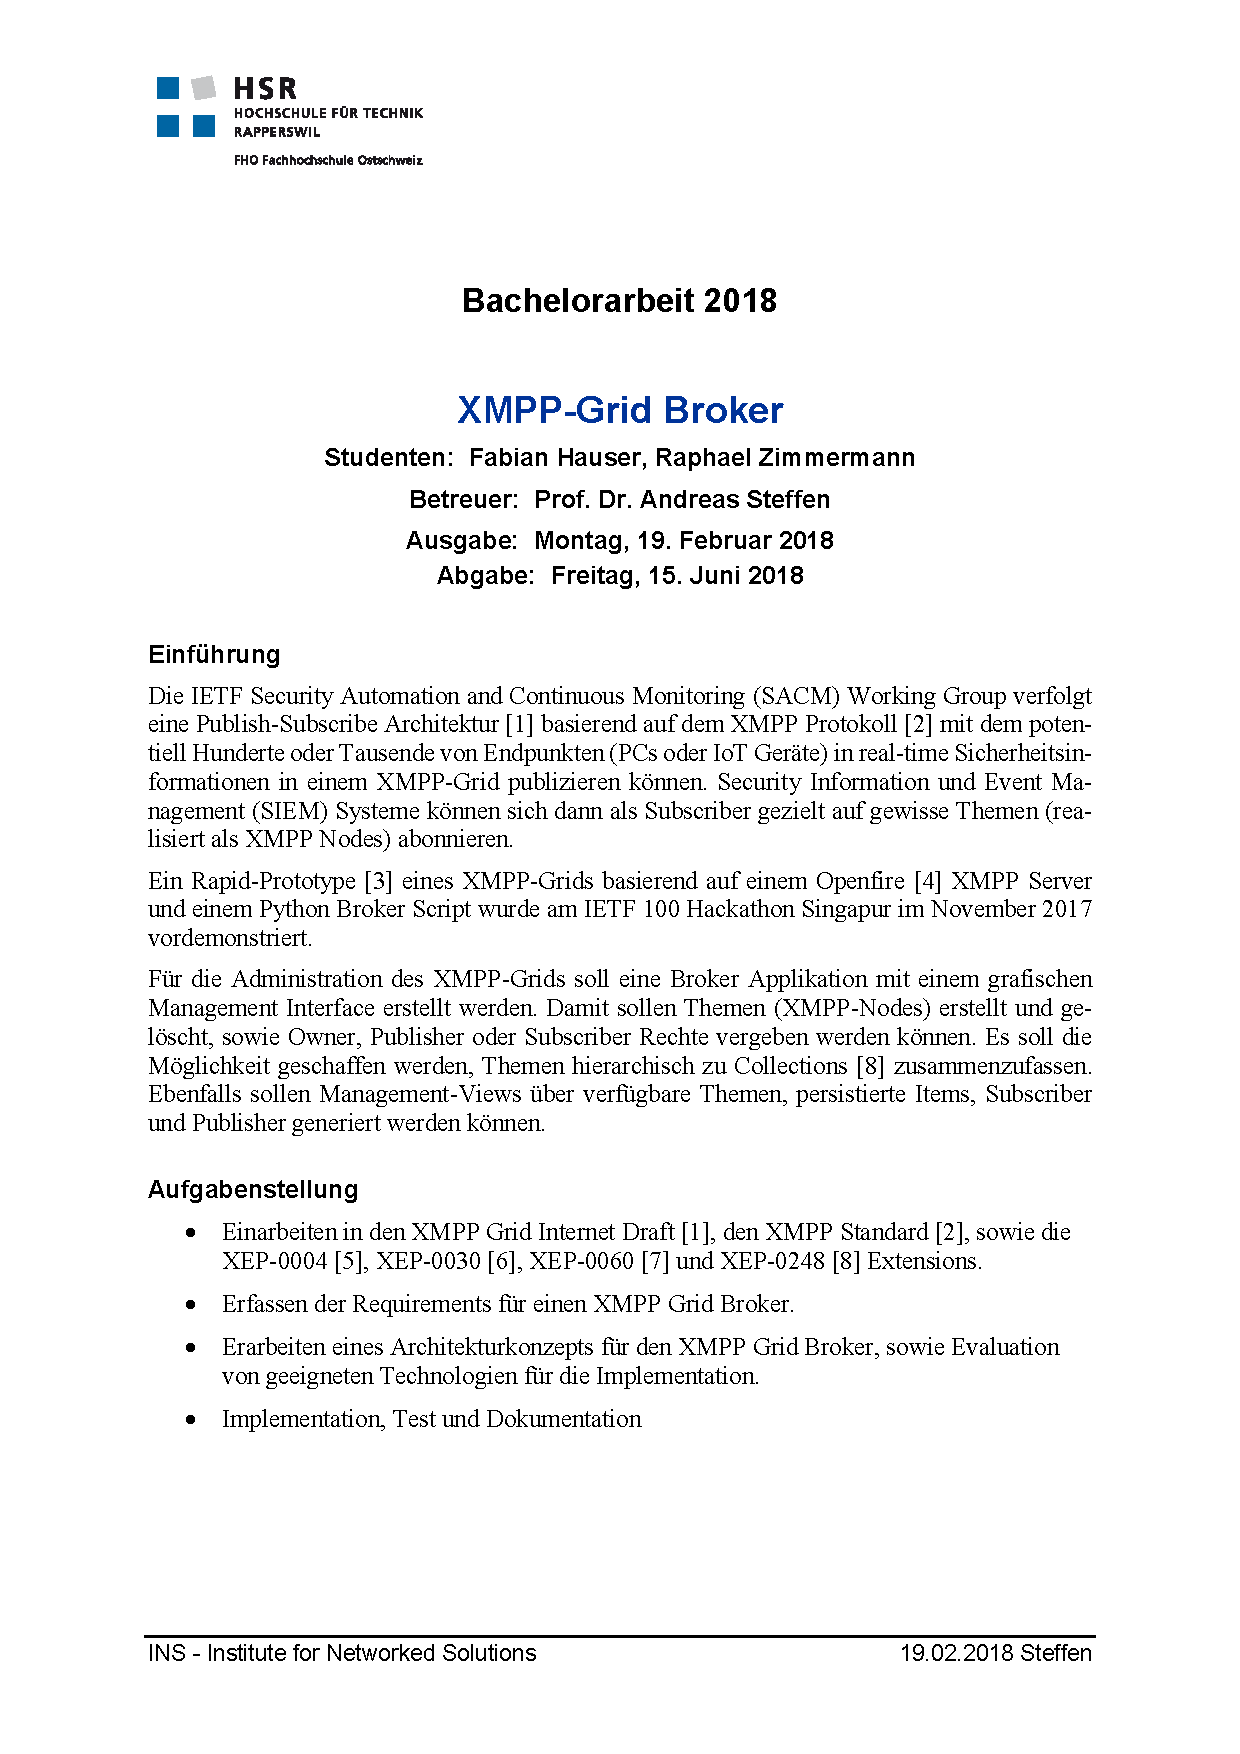
\includepdf[pages=1,scale=.75,frame, pagecommand=\section*{Task Description}\label{sec:task-description}]{../task-description-signed.pdf}
\addchaptertocentry{Task Description}
\includepdf[pages=2-,scale=.75,frame]{../task-description-signed.pdf}

%----------------------------------------------------------------------------------------
%	ABSTRACT PAGE
%----------------------------------------------------------------------------------------

\begin{abstract}
\addchaptertocentry{\abstractname}% Add the abstract to the table of contents
% Context
The IETF Managed Incident Lightweight Exchange~(MILE) working group proposes the standard ``Using XMPP for Security Information Exchange'' which describes how an XMPP based publish-subscribe mechanism (XMPP-Grid) can be used to exchange security-relevant information between network endpoints.\\
\vspace*{1ex}

\noindent
Currently, no implementation of a production-ready and platform-independent administration interface (XMPP-Grid broker) for XMPP-Grids exists.\\
\vspace*{1ex}

%Goal
\noindent
The goal of this thesis is to design and implement an XMPP-Grid broker to configure existing controllers (XMPP servers), focusing on portability, extensibility and the aspects of security in a production environment.
The broker application should enable administrators to configure XMPP-Grids in a usable and productive way.\\
\vspace*{1ex}

%Result
\noindent
Our proposed architecture earmarks a purely client-side web application that communicates with the controller via WebSockets or \gls{http} streams (\gls{bosh}).
The controller is typically protected by a reverse proxy, which also hosts our application.
User logins are performed using mutual TLS authentication to conform to the IETF standard draft.
The resulting application is implemented in TypeScript using the Angular5 framework.\\
\vspace*{1ex}

\noindent
The resulting implementation enables administrators to create and configure communication topics, apprehend the underlying hierarchy and manage permissions.
Additionally, persistent items of topics can be inspected and published.\\
\vspace*{1ex}

% Consequences
\noindent
The XMPP-Grid broker implementation incorporates the specified functionality, resulting in a robust, ready-to-use solution.
A few supplementary helpers, such as autocomplete or filtering, could not be implemented due to limitations of the underlying XMPP standards.
In the future, it will be possible to realise these improvements by enhancing the related XMPP standards or by specifying and implementing proprietary protocols.
\end{abstract}

%----------------------------------------------------------------------------------------
%	MANAGEMENT SUMMARY
%----------------------------------------------------------------------------------------

\chapter{Management Summary}

%The Thesis Management Summary is written here (and usually kept to just this page).
% Das Management Summary richtet sich in der Praxis an die "Chefs des Chefs",
%  d.h. an die Vorgesetzten des Auftraggebers (diese sind in der Regel keine Fachspezialisten).
%  Die Sprache soll knapp, klar und stark untergliedert sein. Zu verwenden ist folgenden Gliederung:
% - Ausgangslage
% - Vorgehen, Technologien
% - Ergebnisse
% - Ausblick (optional)
\section*{Motivation}
The IETF standard draft ``Using XMPP for Security Information Exchange'' describes how devices can exchange security-relevant information within a network, a so-called ``XMPP-Grid'', using the widely adopted messaging protocol ``XMPP''.
Such security-relevant information can be used to take protective measures automatically, e.g. to block devices running outdated software.

An administration interface, referred to as XMPP-Grid broker in the standard draft, is used to configure an XMPP-Grid.
Currently, no such XMPP-Grid broker exists that is production ready and cross-platform.

\section*{Project Goals, Approach}

The goal of this thesis is to engineer an XMPP-Grid broker that allows administrators to configure XMPP-Grids in a straight-forward and productive way.
The resulting application should depend only on the underlying standards and not on specific implementations to support the further standardisation process.

A comprehensive analysis of the underlying standards is carried out in the first part of this thesis.
Particular attention is given to portability, extensibility and aspects of security in a production environment.
This analysis enables a systematic selection of possible architecture options to be executed in the form of architectural decisions.

\section*{Results}

The resulting implementation enables administrators to create and configure communication topics, apprehend the hierarchy of the underlying XMPP-Grid and manage the permissions of network participants.
Additionally, persistent messages can be inspected and published on communication topics.

The XMPP-Grid broker is implemented as an Angular5 web application that connects directly from the web browser to the XMPP-Grid. Secure communication is assured by the use of mutual authentication via TLS.

\section*{Prospects}

The XMPP-Grid broker implementation incorporates the specified functionality, resulting in a robust, ready-to-use solution.
A few supplementary helpers, such as autocomplete or filtering, could not be implemented due to limitations of the underlying XMPP standards.

In the future, it will be possible to realise these improvements by enhancing the related XMPP standards or by specifying and implementing proprietary protocols.

%----------------------------------------------------------------------------------------
%	ACKNOWLEDGEMENTS
%----------------------------------------------------------------------------------------

\begin{acknowledgements}
\addchaptertocentry{\acknowledgementname} % Add the acknowledgements to the table of contents
We would like to thank our advisor, Prof.~Dr.~Andreas~Steffen, for his continuous support and helpful comments.

Tobias~Brunner provided us with valuable feedback on our architecture and introduction section.

Furthermore, we would like to thank Andrea~Jurt~Massey for her feedback regarding writing and language use.
\end{acknowledgements}

%----------------------------------------------------------------------------------------
%	LIST OF CONTENTS PAGES
%----------------------------------------------------------------------------------------

\setcounter{tocdepth}{2}
\tableofcontents % Prints the main table of contents

%----------------------------------------------------------------------------------------
%	DEDICATION
%----------------------------------------------------------------------------------------

%TODO
%\dedicatory{For/Dedicated to/To my\ldots}

%----------------------------------------------------------------------------------------
%	THESIS CONTENT - CHAPTERS
%----------------------------------------------------------------------------------------

\mainmatter % Begin numeric (1,2,3...) page numbering

\pagestyle{thesis} % Return the page headers back to the "thesis" style

% !TeX spellcheck = en_GB
\newcommand{\code}{\texttt}
\chapter{Introduction}
\label{sec:introduction}

\epigraph{Every accomplishment starts with the decision to try.}{unknown}
In this chapter, we present the motivation and legitimisation of our thesis and highlight the scope delimitations.

\section{Motivation}
In this first section, we shall legitimate this thesis and explain the value and applicability of our proposed solution.

\subsection{Present Situation}
The Internet Engineering Task Force (\gls{ietf}) standard draft \emph{Using \gls{xmpp} for Security Information Exchange} \cite{ietf-mile-xmpp-grid-05}, as summarised in section~\fullref{sec:ietf-standard-draft-using-xmpp-for-security-information-exchange}, defines a protocol to exchange security-relevant information between network endpoints.
The draft was created by the Managed Incident Lightweight Exchange (\gls{mile}) working group to support computer and network security incident management.

Hereafter, we refer to this \gls{ietf} standard draft as \gls{xmpp-grid-standard}.

To demonstrate the viability of the \gls{xmpp-grid-standard} a rapid prototype was developed in November~2017~\cite{xmpp-grid-prototype}.

\subsection{Problem and Vision}
Currently, no implementation of the \gls{xmpp-grid-standard} management functionality exists that is ready for production use regarding usability and security.

To solve this problem, a graphical interface with bindings to a suitable \gls{broker} must be proposed and implemented.
The interface should permit network administrators to manage and review \glspl{topic}, \glspl{persisted-item} and \glspl{platform}.
Additionally, \glspl{consumer} and \glspl{provider} permissions of \glspl{topic} and \glspl{platform} must be manageable.

The graphical interface supports administrators to better understand the underlying hierarchy and affiliations of \glspl{topic}, enabling them to assess security implications.
As the interface uses familiar terminology known to an administrator, no in-depth understanding of the underlying \gls{xmpp} technology is required to configure and comprehend an \gls{xmpp-grid}.
Finally, the interface also provides better usability than existing command line interfaces and \gls{xmpp} configuration software, which leads to fewer configuration mistakes and improved efficiency.

We hope that with the help of our implementation the \gls{ietf} draft ``Using \gls{xmpp} for Security Information Exchange'' will become an established security standard used in practical industry applications.

\section{Scope Delimitation} % Abgrenzung
As described in the \nameref{sec:task-description}, the focus of this thesis is on the evaluation, design and implementation of the \gls{xmpp-grid-broker}.
Adding missing functionality or fixing complex bugs in existing server or client implementations are beyond the scope of this thesis.

% !TeX spellcheck = en_GB
\chapter{Analysis}
\epigraph{Without requirements or design, programming is the art\\of adding bugs to an empty text file.}{Louis Srygley}
\section{Terminology}
Taking into account that developers and operators of security reporting systems are the intended audience for this thesis,
we mostly use the  Security Automation and Continuous Monitoring (SACM) terminology~\cite{ietf-sacm-terminology-14}
and thereby follow the same guidelines as the \gls{xmpp-grid-standard}~\cite{ietf-mile-xmpp-grid-05}.

\section{Technical Background}\label{sec:technical-background}

The following sections introduce the \gls{xmpp} protocol including its terminology and summarise the relevant extensions (\glspl{xep}) used by the \gls{xmpp-grid-standard}.

\subsection{XMPP (Extensible Messaging and Presence Protocol)}
The Extensible Messaging and Presence Protocol (in short \gls{xmpp}, formerly known as \gls{jabber}) is an open protocol that enables the near-real-time exchange of small data between any network endpoints, hereafter called \glspl{platform}~\cite{rfc6120}.
While originally designed as an instant messaging (IM) protocol, \gls{xmpp} can be used for a wide range of data exchange applications~\cite{ieee-xplore-stream-xml-xmpp}.

\gls{xmpp} is made of small building blocks defined in the core protocol~\cite{rfc6120} and numerous extensions called \glspl{xep}~\cite{xep-0001}.
The core specifies how encrypted communication channels must be established, how \gls{xml} \glspl{stanza} are exchanged and errors are handled.

The core is comprised of \gls{xml} streams, error handling and functionality for establishing encrypted communication channels.
Additional functionality such as \gls{service-discovery}~\cite{xep-0030} and \gls{publish-subscribe}~\cite{xep-0060} are defined in separate extensions.

Although \gls{xmpp} supports peer-to-peer communication, it is often used in a traditional client-server architecture.
A client (\gls{platform}) can send data to any addressable entity (any other \glspl{platform}) using \Gls{jabber} identifiers, hereafter called \gls{jid}.
If the receiving \gls{jid} has a different domain than the current server (\gls{controller}), the message is forwarded to the \gls{xmpp} server responsible for this domain.~\cite{rfc6120}

The data exchanged over \gls{xmpp} is in the \gls{xml} format, which makes the protocol structured and extensible, but leads to some protocol overhead.
An \gls{xmpp} client communicates with the server over unidirectional data streams, that are basically long-lived \gls{tcp} connections.
A client opens a channel to the server over this connection, and the server reacts by opening a connection in the opposite direction.
In both streams, an XML document is opened after the connection is established (i.e. with \code{<stream>} XML tags).
During the conversation, an arbitrary amount of \glspl{stanza} (specified XML child elements) are written to the stream.
Before a connection may be terminated, the root element is closed (i.e. \code{</stream>}) and both streams form valid XML documents~\cite{rfc6120, professional-xmpp}.

The core \gls{stanza} types are \glspl{message}~(\code{<message/>}), \gls{presence}~(\code{<presence/>}) and\\
\gls{info-query}~(\code{<iq/>}).
\Glspl{message} can contain arbitrary data similar to email but are optimised for immediate delivery.
\Gls{presence} \glspl{stanza} deal with network availability and the propagation of user presence information.
An \gls{info-query} \gls{stanza} consists of a request and response (similar to the GET and POST \gls{http} methods), which is used for feature negotiation, configuration and general information exchange.
Because of these coarse semantics, \gls{xmpp} provides a generalized communication layer~\cite{rfc6120, ieee-xplore-stream-xml-xmpp}.

Figure~\ref{fig:xmpp-overview} illustrates an example setup with two servers and three clients.

\begin{figure}[h]
	\centering
	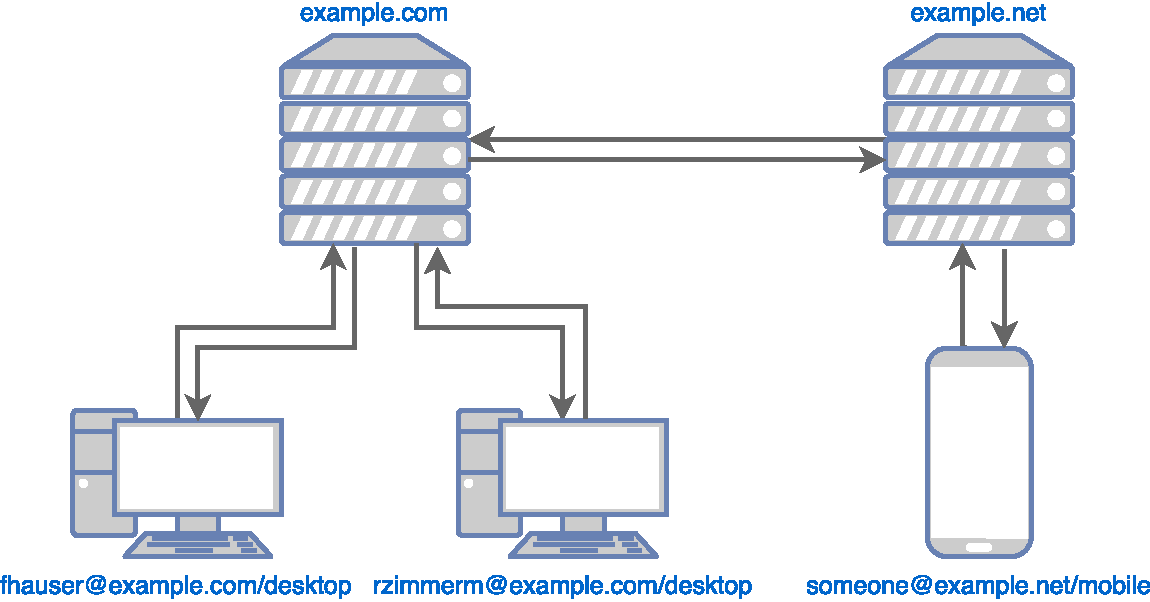
\includegraphics[width=0.8\linewidth]{resources/xmpp_overview.pdf}
	\caption[XMPP example overview]{Two \gls{xmpp} domains (servers), one with two users and one with a single mobile user.}
	\label{fig:xmpp-overview}
\end{figure}

\subsection{Relevant XMPP Extensions}

The \gls{xmpp-grid-standard} is based on multiple \glspl{xep}, most notably the \gls{publish-subscribe} extension. In this section, we give an overview of the most relevant used \glspl{xep}.

\paragraph{XEP-0004: Data Forms} is a flexible protocol that can be used in workflows such as service configuration.
The protocol provides form processing, common field types and extensibility mechanisms.~\cite{xep-0004}

\paragraph{XEP-0030: Service Discovery} enables entities to discover information about the identity and capabilities of other entities, e.g. whether the entity is a server or not, or items associated with an entity, e.g. a list of \gls{publish-subscribe} nodes.~\cite{xep-0030}

\paragraph{XEP-0059: Result Set Management} allows entities to manage the receipt of large result sets, e.g. by paging through the result or limiting the number of results. \gls{result-set-management} is often desired when dealing with large dynamic result sets, as from service discovery or publish-subscribe, and when time or other resources are limited.~\cite{xep-0059}

\subsubsection{XEP-0060: Publish-Subscribe}
The \gls{publish-subscribe} extension, hereafter referred to as \gls{pubsub} or \gls{broker}, enables \gls{xmpp} entities (\glspl{provider}) to broadcast information via \glspl{topic} to subscribed entities (\glspl{consumer}).~\cite{xep-0060}

Nodes, hereafter referred to as \glspl{topic}, are the communication hubs. Entities can create \glspl{topic} and configure them, e.g. set up subscription timeouts or limit publishing and subscription rights. The configuration mechanism is based on data forms (XEP\babelhyphen{nobreak}0004).
An \gls{xmpp} server \emph{may} restrict \gls{topic} creation to certain entities, which means that possibly not every \gls{xmpp}-Server that supports \gls{publish-subscribe} also implements this feature \cite{rfc2119}.

The protocol defines a hierarchy of six affiliations of which only the implementation of owner and none is \emph{required}.
Implementing the remaining four affiliations is \emph{recommended}.
An owner of a \gls{topic} can manage the subscriptions and affiliations of other entities associated with a given \gls{topic}.

To simplify the creation of \glspl{topic}, \gls{pubsub} defines five \gls{topic} access models (node access models) that \emph{should} be available: open, presence, roaster, authorize and whitelist.
The open model allows uncontrolled access while presence and roaster are specific for IM. Using the authorize model, the owner has to approve all subscription requests.
The whitelist model enables the owner to maintain a list of entities that are allowed to subscribe.


\section{Domain Analysis}

\subsection{IETF Standard Draft: Using XMPP for Security Information Exchange}\label{sec:ietf-standard-draft-using-xmpp-for-security-information-exchange}
This \gls{ietf} standard draft describes how the \gls{xmpp} protocol and its extensions can be used for the exchange and distribution of security-relevant information between network devices.

One of the primary motivation for using \gls{xmpp} for this task is the fast propagation of such security-relevant data.
Using \gls{xmpp} for such a task also comes with its downsides. Most notably, because the \gls{xmpp} server (\gls{broker}/\gls{controller}) is the central configuration component in charge of managing access permission, its compromisation has serious consequences.

The standard describes a trust model, a thread model as well as specific countermeasures, e.g. to use at least \gls{tls} 1.2. These countermeasures also define restrictions of the \gls{xmpp} protocol and its extensions, e.g. by limiting the \gls{topic} access models of \gls{pubsub} to whitelist and authorized only~\cite{ietf-mile-xmpp-grid-05}.

\subsubsection{Information Exchange Format}

The \gls{xmpp-grid-standard} states that `although [the exchanged] information can take the form of any structured data (XML, JSON, etc.), this document illustrates the principles of \gls{xmpp-grid} with examples that use the Incident Object Description Exchange Format (IODEF)'~\cite{rfc7970, ietf-mile-xmpp-grid-05}.

As IODEF is not strictly defined nor explicitly recommended by the \gls{xmpp-grid-standard}, no specific integrations are in the scope of this thesis.

In practice, small payloads are sent over an \gls{xmpp-grid}, usually containing external pointers to an API that provides more comprehensive data (see appendix~\fullref{sec:meeting-minutes}).

\subsection{Domain Specific Language}

Figures~\ref{fig:architecturedslgriddraft} and \ref{fig:architecturedslxeps} present an overview of the relevant interactions and relationships between the different components as specified in the \gls{xmpp-grid-standard} and the referenced \glspl{xep} (see section~\fullref{sec:technical-background}).

\begin{figure}[h]
\centering
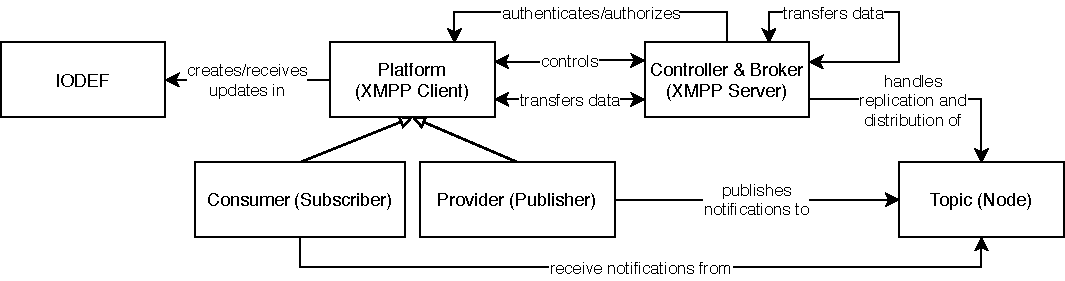
\includegraphics[width=\linewidth]{resources/architecture_dsl_grid_draft}
\caption[DSL of the XMPP-Grid standard]{Domain specific language of the \gls{xmpp-grid-standard}.}
\label{fig:architecturedslgriddraft}
\end{figure}

\begin{figure}[h]
\centering
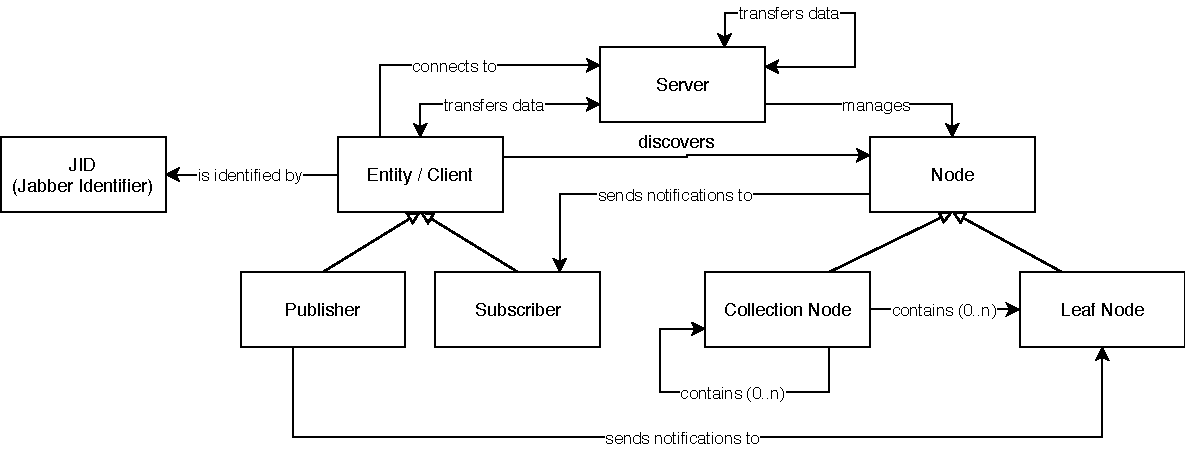
\includegraphics[width=\linewidth]{resources/architecture_dsl_xeps}
\caption[DSL of used XMPP XEPs]{Domain specific language of used \gls{xmpp} \glspl{xep}.}
\label{fig:architecturedslxeps}
\end{figure}

\section{Requirements Analysis}

We collected the functional requirements in the form of user stories.
User stories are an established and widespread concept for describing and managing requirements in agile software projects.
In comparison to traditional tools for requirement analysis, user stories are more concise, leaving more space for change. \cite{wirdemann2017scrum}

We also created user stories for non-functional requirements.
Additional non-functional requirements can be added during the project in the form of constraints. \cite{wirdemann2017scrum}

In the early phase of the project, we collected an initial set of user stories in collaboration with Prof.\ Dr.\ Steffen.
This initial set covered the creation and deletion of \glspl{topic} as well as  granting publish and subscribe privileges.
All user stories are listed in appendix~\fullref{sec:requirements}.

After setting broad priorities, Prof.\ Dr.\ Steffen approved the initial set of user stories that then served as the basis for the architectural concept.
% !TeX spellcheck = en_GB
\chapter{Concept} % Lösungsentwurf 
\epigraph{Perfection (in design) is achieved not when there is nothing more to add,\\but rather when there is nothing more to take away.}{Antoine de Saint-Exupery}

\section{Architecture}\label{sec:architecture}

In this section, we present the architecture and fundamental architectural decisions of the \gls{xmpp-grid-broker} application.
All architectural decisions we took are fully documented in appendix~\fullref{sec:architectural-decisions}.

We illustrate the concepts and structures using the C4 Model for Software Architecture~\cite{c4-model}.

\subsection{Actors and Context}

The context diagram pictured in figure~\ref{fig:architecturecontext} shows the actors and surrounding systems that are given for the \gls{xmpp-grid-broker}, as described in the \nameref{sec:task-description}.

One or more administrators manage the \gls{xmpp-grid} by adding or removing \glspl{platform} and configuring \glspl{topic}.
To minimize the required work and reduce the error-proneness, administrators interact with the \gls{xmpp-grid-broker}.

The \gls{xmpp-grid-broker} configures the \gls{xmpp-grid}, which consists of a \gls{controller} and \glspl{platform}.

\begin{figure}[h]
\centering
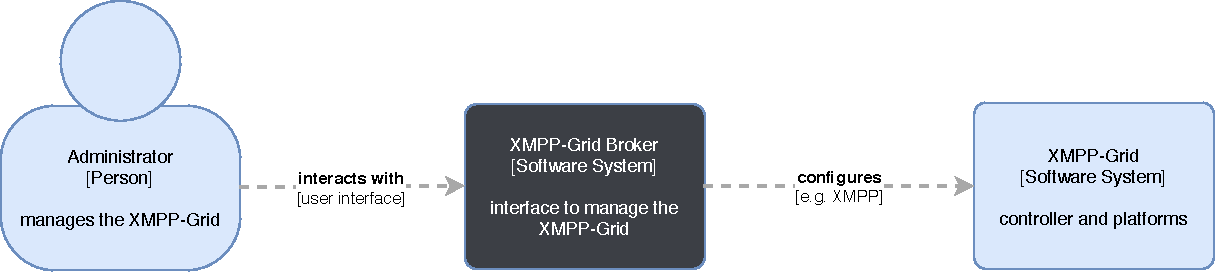
\includegraphics[width=\linewidth]{resources/architecture_context}
\caption[Architecture context diagram]{Architecture diagram showing the context of the \gls{xmpp-grid-broker} application.}
\label{fig:architecturecontext}
\end{figure}


\subsection{Architectural Style}

To implement the \gls{xmpp-grid-broker}, we evaluated three possible architecture styles:\hfill\\
An \gls{xmpp} server plug-in (e.g. extension for the Openfire \gls{xmpp} server), an implementation using the Jabber Component Protocol~\cite{xep-0114} and an implementation acting as a regular \gls{xmpp} client ("bot").

We decided to build an \gls{xmpp} client/bot because, unlike a server plugin, it is not coupled to a specific \gls{xmpp} server.
In contrast to the \gls{xmpp} component, \gls{xmpp} clients support strong authentication mechanisms with \gls{sasl}.

The full decision argument is documented in appendix~\fullref{sec:architectural-decisions}.

\subsection{Platform}

The proposed \gls{xmpp} client might be implemented in different ways: as rich client application with a command line or graphical interface as illustrated in figure~\ref{fig:architecturecontainerrichclient}, and in the form of a web application, illustrated in figures~\ref{fig:architecturecontainerwebapplication} and \ref{fig:architecturecontainerwebproxy}.

\subsubsection{Rich Client Application}

The idea of a rich client application is to communicate directly from a graphical desktop application with the \gls{xmpp-grid}, as illustrated in figure~\ref{fig:architecturecontainerrichclient}.

\begin{figure}[h]
\centering
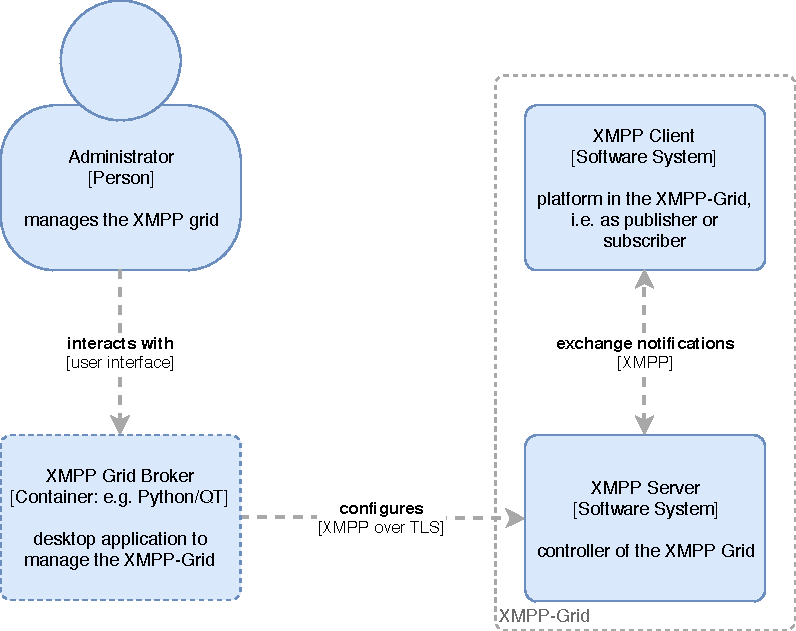
\includegraphics[width=0.7\linewidth]{resources/architecture_container_rich_client}
\caption[Architecture container diagram: Rich client]{Architecture container diagram showing a possible rich client architecture.}
\label{fig:architecturecontainerrichclient}
\end{figure}

\subsubsection{Web Application}

In contrast to a rich client application, a web application has the significant advantage to be easily installable and upgradable with minimal interaction on the user's side (i.e. only requires a web browser to be executed).

Therefore, we decided to implement the \gls{xmpp-grid-broker} as web application.

To manage the \gls{controller} from the \gls{broker} interface, we considered either directly connecting to the \gls{xmpp} server over WebSockets~\cite{rfc7395} or \gls{http} (\gls{bosh}~\cite{xep-0124}), and the indirect communication with the \gls{xmpp} server via custom web API proxy.
These topologies are illustrated in figure~\ref{fig:architecturecontainerwebapplication} and figure~\ref{fig:architecturecontainerwebproxy}.

\begin{figure}[h]
\centering
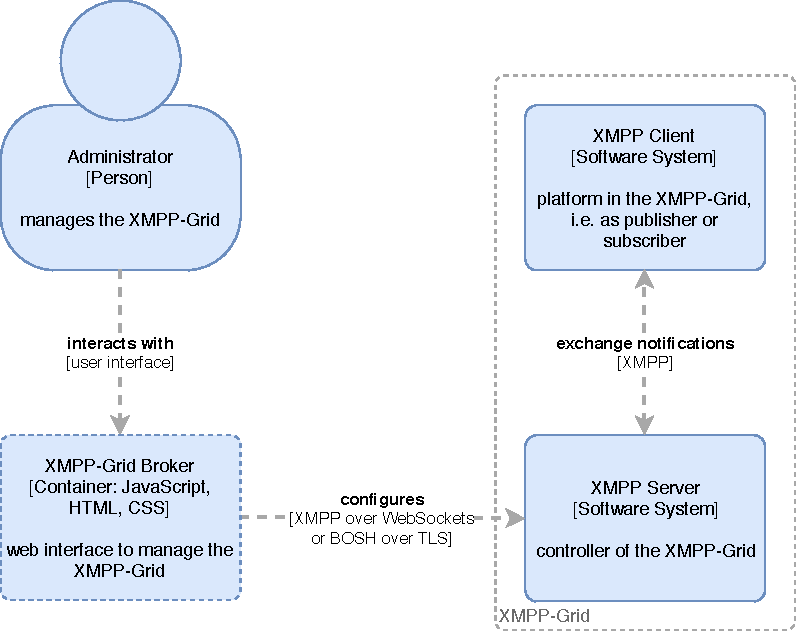
\includegraphics[width=0.7\linewidth]{resources/architecture_container_webapplication}
\caption[Architecture container diagram: Web application]{Architecture container diagram showing the web application topology with WebSockets or \gls{bosh}.}
\label{fig:architecturecontainerwebapplication}
\end{figure}

\subsubsection{Web API Proxy}

A web API proxy could be realised with a custom browser-to-proxy protocol, as implemented in the \gls{xmpp}-FTW JavaScript library\footnote{\url{http://docs.xmpp-ftw.org/}}.
However, this approach leads to a high coupling between a concrete library and the web application.

Another approach would be the implementation of a custom WebSocket-to-\gls{xmpp} Proxy, which allows connecting to \gls{xmpp} servers that do not support WebSockets or \gls{bosh}.
If such a proxy is implemented transparently, the client is not aware of the server limitations.
Therefore, the client implementation is no different from direct communication with an \gls{xmpp} server.

As the \gls{xmpp} over WebSocket protocol differs from the normal \gls{xmpp} protocol, a transparent proxy implementation would inevitably need to hold the connection state and implement custom keep-alive mechanisms~\cite{rfc7395}.

\begin{figure}[H]
\centering
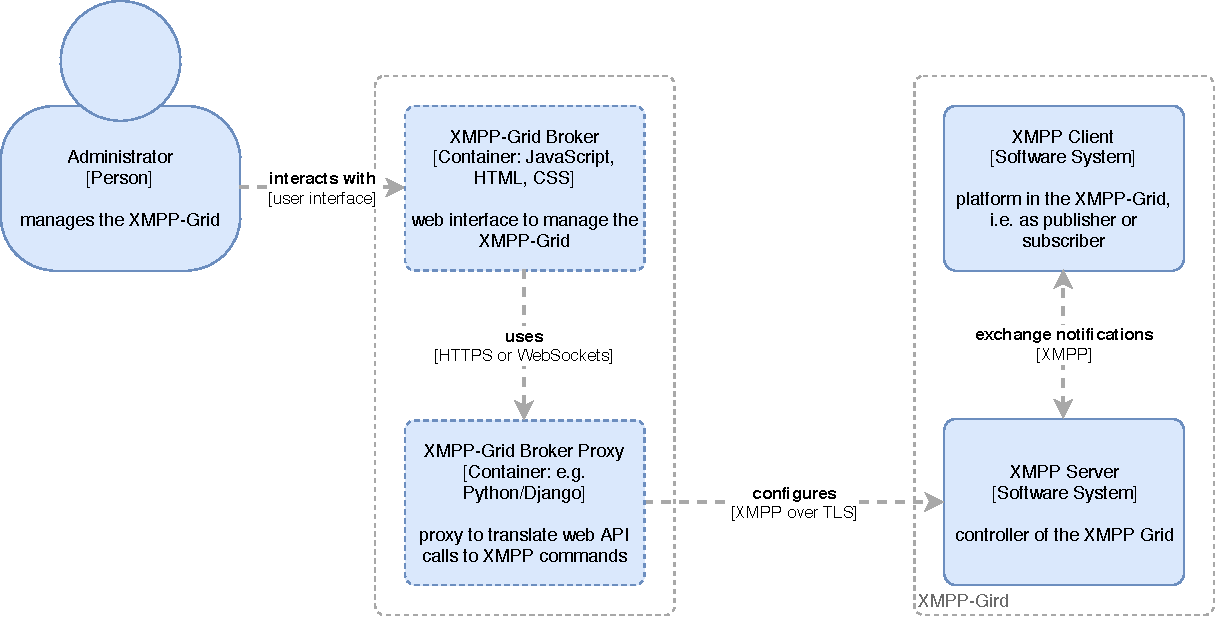
\includegraphics[width=0.8\linewidth]{resources/architecture_container_proxy}
\caption[Architecture container diagram: Web proxy]{Architecture container diagram showing the web API proxy topology.}
\label{fig:architecturecontainerwebproxy}
\end{figure}

\subsubsection{Implemented Web Application Topology}\label{sec:implemented-web-application-topology}

As described in the according architectural decision (see appendix~\fullref{sec:architectural-decisions}), we decided on the option that connects directly via WebSockets, if possible with a fallback to \gls{bosh}.
This topology simplifies the implementation and deployment of the application in comparison to a web API proxy.
WebSockets offer stateful \gls{tcp}-sockets to exchange data with \gls{xmpp} servers in contrast to \gls{bosh}, which uses \gls{http} long polling to emulate bidirectional streams and is, therefore, less efficient~\cite{xep-0124}.

To increase the \gls{xmpp} server security, an \gls{http} reverse proxy (e.g.\ nginx\footnote{\url{https://nginx.org/}}) between the client and the \gls{xmpp} server might be added as shown in figure~\ref{fig:architecturecontainerweb-http-proxy}.
The reverse proxy might also be used to serve the web application and provide authentication (see section~\fullref{sec:authentication-and-connection-security}) and security features (see section~\fullref{sec:ops-security}).

\begin{figure}[H]
    \centering
    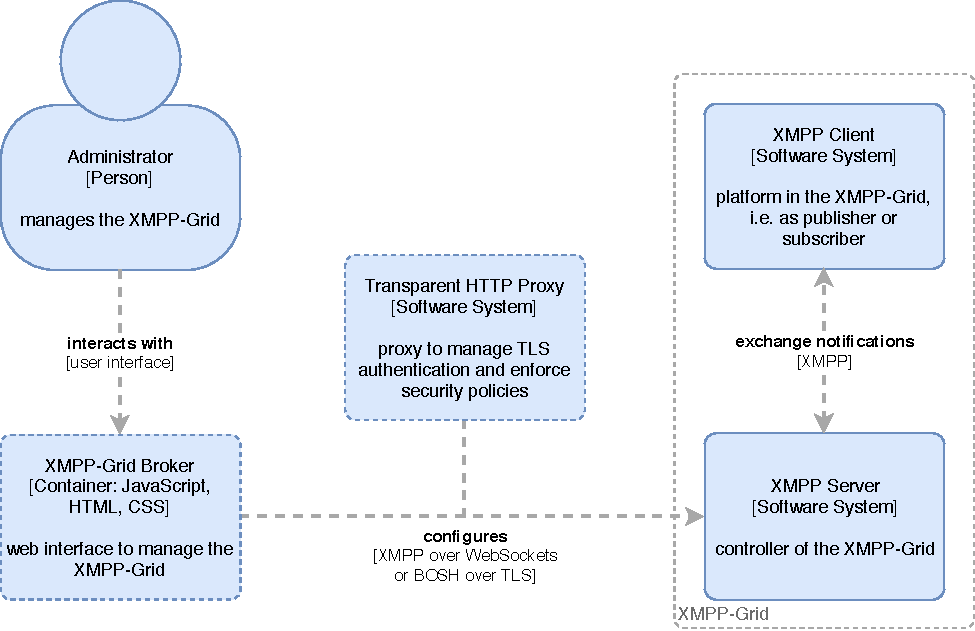
\includegraphics[width=\linewidth]{resources/architecture_container_webapplication_with_http_proxy}
    \caption[Architecture container diagram: Web application with proxy]{Architecture container diagram showing the implemented web application topology.}
    \label{fig:architecturecontainerweb-http-proxy}
\end{figure}
  

\subsection{Authentication and Connection Security}\label{sec:authentication-and-connection-security}

\gls{xmpp} uses \gls{sasl} as authentication mechanism~\cite{rfc6120}.
To authenticate against the \gls{xmpp-grid} \gls{controller}, we decided to use the \gls{sasl-external}~\cite{rfc4422} mechanism whenever possible to authenticate the client.

We decided against \gls{sasl-scram}~\cite{rfc7677}, the alternative authentication method that is also recommended by in the \gls{xmpp-grid-standard}.
As described in the corresponding architectural decision (see appendix~\fullref{sec:architectural-decisions}), the main reason for \gls{sasl-external} is its higher level of security and and its relatively simple scaling capabilities.

\gls{sasl-external} implies that the authentication takes place on a lower layer than the actual \gls{xmpp} protocol. In our case, this implies authentication over \gls{tls}, i.e.~X.509 user certificates as specified in RFC6120~\cite{rfc6120}.

Currently, not all \gls{xmpp} servers that implement \gls{bosh} and Websockets also implement \gls{sasl-external} with \gls{tls} authentication
(e.g.\ Openfire currently supports \gls{tls} authentication with \gls{bosh} but not with Websockets\footnote{\url{https://github.com/igniterealtime/Openfire/blob/02c22e/src/java/org/jivesoftware/openfire/websocket/OpenfireWebSocketServlet.java}}).
To circumvent this limitation, an \gls{http} reverse proxy (see section~\fullref{sec:implemented-web-application-topology}) might be used to handle \gls{tls} authentication.

\subsection{Concurrency, Scalability and Performance}

As presented in the architecture above, the \gls{broker} application communicates directly from the user's web browser with the \gls{xmpp} server.
By adopting this approach, the main scalability concern is on the \gls{xmpp} server.
This approach is also in alignment with the \gls{xmpp} philosophy to move as much complexity as possible on the server \cite{definitive-guide-xmpp}.

Concurrency and scalability are the responsibility and speciality of the underlying \gls{xmpp} server and therefore not directly relevant for the \gls{broker} application \cite{definitive-guide-xmpp}.

Regarding performance, the network is the primary source of potential slowdowns.
The \gls{xmpp-grid-broker} must reduce the number of requests needed to a minimum and whenever possible execute requests in parallel.
Additionally, the initial loading time of the application can be optimised.

A potentially used reverse proxy must be scaled with the number of administrators.
As this number is usually rather small, no extra effort is usually required.

\section{Wireframes}

We created wireframes for most screens to visualise the initial set of user stories.
They helped us to find missing requirements, most notably the support of collections.
All wireframes are listed in appendix~\fullref{sec:wireframes}.

\section{Security Considerations}\label{sec:security-considerations}

Regarding the \gls{xmpp-grid-broker} application, there are three primary attack vectors:

\begin{description}
    \item[Client-Side Attacks,] e.g. via web browser, web browser extension or malicious software on the client operating system.
    \item[Web Server Attacks,] e.g. misconfiguration or insufficient hardening.
    \item[\gls{xmpp} Server Attacks,] e.g. misconfiguration or insufficient hardening.
\end{description}

Details on all these attack vectors are discussed in the following sections.

\subsection{The XMPP Protocol}

An in-depth security analysis of the \gls{xmpp} protocol is beyond the scope of this thesis.
A detailed discussion of security concerns can be found in the \gls{xmpp} specification~\cite{rfc6120} and most XEPs~\cite{xep-0060, xep-0248}.
In this section, we highlight the most crucial security concerns relevant to this thesis.

\subsubsection{Transport Security}

\gls{xmpp} reuses many established and standardised mechanisms to improve protocol security.
By layering protocols in a strict manner (\gls{xmpp} with \gls{sasl} over \gls{tls} over \gls{tcp}), many attack scenarios such as replaying or eavesdropping are minimised.
The protocol also requires clients and servers to validate the certificates of the other party.~\cite{rfc7590, rfc6120}

\subsubsection{Protocol}

Since \gls{xmpp} is based on XML, it inherits some of its security implications.
\gls{xmpp} prohibits some XML features such as comments and external entity references which mitigate common attacks.~\cite{rfc6120}

The protocol itself cannot mitigate attacks where an attacker gains access to account credentials.
To reduce the risk of these attack vectors best practices such as storing certificates and passwords securely must be followed.

\subsubsection{PubSub Collection Nodes}

The use of XEP-0248 PubSub Collection Nodes~\cite{xep-0248} can leak private data if not configured properly.
Administrators must take great care when configuring collection nodes.
The \gls{xmpp-grid-broker} should support administrators to detect such data leaks.

\subsection{Client Security}

Because the web gives rise to many potential security concerns, above all a modern web browser is critical for client security.
Legacy web browsers can not provide an adequate level of security.~\cite{firefox-update-security}

Most web browsers support extension mechanisms which have rather significant capabilities~\cite{browser-extension-security}.
The usage of untrusted and uncertified browser extensions is strictly discouraged.

The same applies to the client operating system and all software installed on clients.

\subsubsection{Authentication and Authorisation}

Regarding authentication and authorisation, the \gls{xmpp} server does most of the heavy lifting such as storing passwords and validating certificates.
On the client side, the web browser does most of that work too (i.e. validating certificates).

The responsibility of a client implementation is to establish a secure channel to the \gls{xmpp} server and warn the user if a problem occurs during this process (e.g. invalid server certificate).

\subsubsection{Angular Framework}

Using the Angular framework impacts client security significantly.
Angular is built with security in mind and is adopted in the industry in security-relevant environments.
Therefore, Angular receives frequent security updates and is well tested.
It's unlikely that a similar security level might be reached with plain JavaScript in a reasonable implementation timespan.

On the project website, three best practices regarding security are recommended~\cite{angular-security}.

\begin{itemize}
    \item Keep up with the latest Angular library releases.
    \item Don't modify your copy of Angular.
    \item Avoid Angular APIs marked in the documentation as ''Security Risk''.
\end{itemize}

We can ensure the latter two by making them acceptance criteria.
Keeping current with the latest Angular releases is harder, as our work on this project is limited.
To ensure that future updates can easily be applied we deviate as little as possible from the standard angular setup (e.g. by not ejecting the Webpack configuration\footnote{\url{https://github.com/Angular/Angular-cli/wiki/eject}}).

Keeping Angular up-to-date is of paramount importance as potential vulnerabilities (e.g. XSS) can be exploited if not patched.

\subsubsection{Angular Content Security}

Except for \glspl{persisted-item}, no \gls{xmpp} content is displayed directly but serves as the basis for rendered HTML components.
To protect against malicious payloads, the received XML messages must be validated before their usage.

\Glspl{persisted-item} can contain arbitrary content and must therefore be escaped before rendering to prevent Cross-Site Scripting (XSS) attacks.

Angular supports these measures by treating all values (except Angular templates) as untrusted by default.
To prevent user-generated data to influence Angular templates, the offline template compiler is used. To fully utilise the security measures provided by Angular, official APIs must be used at all times instead of direct use of the DOM-APIs.~\cite{angular-security}

Using Content-Security-Policy (CSP) provides additional XSS-protection mechanisms \cite{w3c-csp}.
The \gls{xmpp-grid-broker} should document an appropriate CSP that must be supported in a production environment.

\subsection{Server Security}

\subsubsection{Authentication and Authorisation}

The \gls{xmpp} server implements most of the authentication and authorisation mechanisms used in an \gls{xmpp-grid-broker} implementation, such as storing passwords and validating certificates.

If \gls{bosh} or WebSockets are used, the \gls{xmpp} server should support most \gls{http} security features as listed in section~\fullref{sec:web-server}. Additionally, the origin of WebSockets and \gls{bosh} requests must be verified (by either the Origin header or CORS support.~\cite{rfc6455, cross-origin-resource-sharing}

The web server hosting the client application has no active authentication or authorisation responsibility, except to ensure the integrity and authenticity of the application, i.e. by using \gls{tls}.

\subsubsection{Web Server}\label{sec:web-server}

To minify security concerns on the server side, we decided to keep the application files static (see \fullref{sec:architectural-decisions}).
This allows operators to use any standard web server (e.g. nginx, Apache, etc.) to serve the client.
Securing such standard web servers is common knowledge for operators and is beyond the scope of this analysis.

In addition to these general best practices, we explicitly recommend the following security measures to improve client security:

\begin{itemize}
    \item Enable Content Security Policy (CSP)~\cite{w3c-csp}.
    \item Use secure \gls{tls} configurations such as secure cipher suites, strictly honor cipher order, HSTS, HPKP and OCSP Stapling\cite{mozilla-tls-recommendations}.
\end{itemize}

These recommendations should be documented in the application installation guide.

\subsubsection{XMPP Server}

\gls{xmpp} server security depends on the chosen implementation and the application domain.
Discussing \gls{xmpp} server security in detail is beyond the scope of this thesis.
Operators should adhere to the security recommendations of their \gls{xmpp} server vendor and follow general security best practices as outlined by the \gls{xmpp-grid-standard}.

\section{Security Risk Mitigation}\label{sec:security-risk-mitigation}

To mitigate the security risks as discussed in section~\fullref{sec:security-considerations}, the measures as described in the following subsections are implemented.

\subsection{Development}

\begin{enumerate}
    \item Conduct code reviews for all newly added code using GitHub pull requests and a security checklist (see next section)
    \item Conduct an architectural analysis with an industry expert\footnote{Was carried out on 2018-04-16, see \fullref{sec:meeting-minutes}.}
    \item Automate build and release processes to minimise the time required to patch
    \item Stay as close to the default Angular setup to simplify further updates
    \item Avoid additional third-party dependencies whenever possible
\end{enumerate}

\subsection{Client Security Checklist}
\begin{itemize}
    \item The latest Angular-version is used
    \item No customizations are made to the Angular version
    \item No direct access to DOM-APIs
    \item APIs marked in the documentation as ``Security Risk'' are \emph{not} used
    \item No usage of any methods starting with \code{bypassSecurityTrust}
    \item The client is fully Content Security Policy (CSP) compliant
    \item The client is fully Same Origin Policy (SOP) / Cross-Origin Resource Sharing (CORS) compliant
    \item Only compile templates with the offline template compiler (AOT)
    \item User input is always escaped using the mechanisms provided by the framework (eg. Angular Forms)
    \item \gls{xmpp} messages are validated to contain only the specified result-types
\end{itemize}


\subsection{Operations Security}\label{sec:ops-security}

Administrators must configure the surrounding systems correctly to mitigate certain security risks.
To support administrators, we recommend the following measures.

\subsubsection{Content Security Policy}

The Content Security Policy (CSP) helps to mitigate certain types of attacks such as Cross Site Scripting (XSS) as a second line of defence \cite{w3c-csp}.
The recommended values are directly documented in the project source code repository.

\subsubsection{Verify Origin}
The \gls{xmpp} server should be configured to only accept WebSockets/\gls{bosh} connections from the origin of the \gls{xmpp-grid-broker} application.
The Origin header sent by the web browser must match the domain on which the \gls{xmpp-grid-broker} application is hosted.
Otherwise, connection requests must be ignored.
If an \gls{xmpp} server does not support this feature, a proxy server should be used to verify the Origin header.
In the provided development setup, this security feature must not necessarily be implemented.

% !TeX spellcheck = en_GB
\chapter{Implementation and Testing} % Realisierung und Test
\epigraph{Any fool can write code that a computer can understand. Good programmers write code that humans can understand.}{Martin Fowler}


\section{Development Setup}\label{sec:development-setup}

Figure~\ref{fig:development-setup} illustrates the development setup in the form of an UML deployment diagram.
Developers connects from their browsers to the reverse proxy that serves the static \gls{broker} web application.
The \gls{http} connection from the client to the server is secured using mutual \gls{tls} authentication.
The same reverse proxy also routes the \gls{xmpp} connections.
The proxy establishes a mutual authenticated \gls{tls} connection to the \gls{xmpp} server.
The reasons for this setup are described in more detail in section~\fullref{sec:limitations-of-the-openfire-xmpp-server}.

\begin{figure}[h]
    \centering
    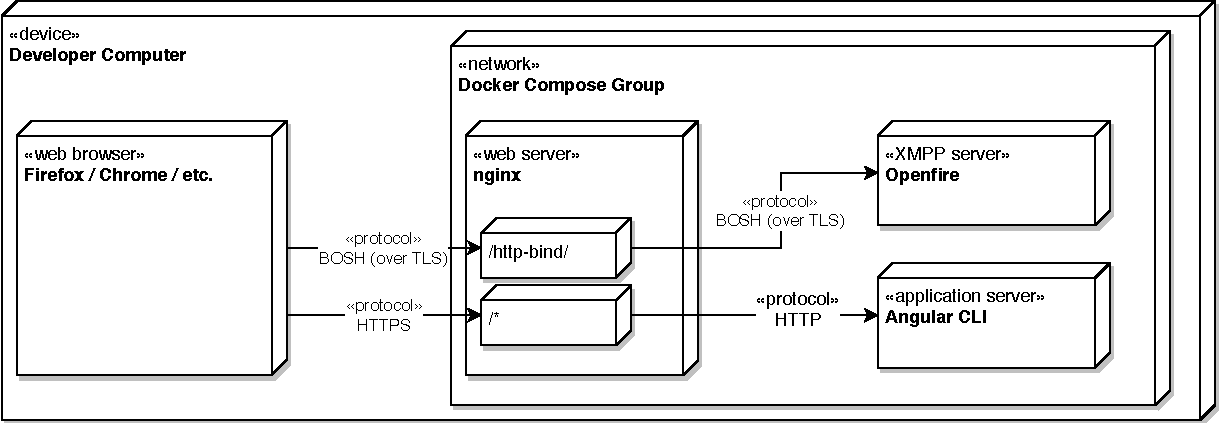
\includegraphics[width=1\linewidth]{resources/development-setup-uml}
    \caption[Development setup deployment diagram]{UML deployment diagram presenting the development setup.}
    \label{fig:development-setup}
\end{figure}

As the previously described structure is not trivial, the guiding principle for our development setup was to maximise automation and minimise manual efforts.
This principle is the basis for durable software.
We decided on a docker and docker-compose\footnote{\url{https://www.docker.com/}} based stack that provides a correctly configured Openfire instance, a preconfigured nginx instance as well as client and server certificates.
Everyday tasks such as building and testing the application and documentation were automated as bash scripts.

The efforts invested in this docker setup proved valuable when we began to write integration tests that run in the same environment.

We deliberately decided to run unit tests outside of the docker environment as unit tests are executed more often, and the additional docker-overhead would be unnecessarily expensive.
Also, debugging is more straightforward without indirections.

\section{Encountered Problems}\label{encountered-problems}

\subsection{Multiple Administrators}\label{sec:limitations-of-requirement-multiple-administrators}

Requirement \fullref{sec:requirement-multiple-administrators} states that multiple administrators should be able to access the application.

When authenticating users with \gls{sasl-external}, the client certificate extension field xmppAddr is interpreted as user \gls{jid} by the \gls{xmpp} server.

In practice, most \gls{xmpp-grid-broker} deployments require an \gls{http} proxy in front of the \gls{xmpp} server as security measure (see section~\fullref{sec:implemented-web-application-topology}).
Usually, the \gls{http} proxy can also be used to serve the \gls{broker} application, as realised in the development setup.
Such an \gls{http} proxy might also accept multiple client certificates.

If the client connects to the \gls{xmpp} server over secure WebSockets (WSS) in combination with \gls{sasl-external}, the WebSocket URL must already be authenticated, as most browsers do not permit certificate selection on background requests~\cite{chromium-issue-background-certs}.
This might be achieved by serving the \gls{broker} from the same domain or by using client certificate policies~\cite{chrome-cert-policies}.

As the proxy intercepts the \gls{tls} connection, it must verify the client certificate sent by the browser and establish a connection to the \gls{xmpp} server using a client certificate as well.
Therefore, the xmppAddr field of the proxy's client certificate is used by the \gls{xmpp} server.
If multiple users should be differentiated on the \gls{xmpp} server, an \gls{http} proxy might choose different client certificates for connecting to the \gls{xmpp} server based on the web browser's client certificate xmppAddr.


\subsection{Audit Trails}

Actions of administrators should be traceable with an audit trail according to requirement \fullref{sec:requirement-audit-trail}.

As outlined in section~\fullref{sec:limitations-of-requirement-multiple-administrators}, practical deployments of \glspl{xmpp-grid-broker} mostly use an \gls{http} proxy.
The proxy can also be used to keep an audit trail of client requests.
These requests can then be correlated with the query log on the \gls{xmpp} server.

Audit trails on the client side are not trustworthy, as users might prevent trail entries by manipulating the client application.
Therefore, no such mechanism was implemented.

\subsection{Logout}

Administrators should be able to terminate a session by using a logout function, as stated in requirement~\fullref{sec:requirement-logout}.

We decided to use \gls{tls} client certificate authentication as part of \gls{sasl-external}.
As a result of our decision to write a web application, the web browser authenticates users with \gls{tls} certificates.

Unfortunately, web browsers do not expose a standardised way to log out of a \gls{tls} client authenticated session \cite{practical-issues-with-tls-client}.
To close the \gls{tls} session, administrators must close their browser window after using the \gls{xmpp-grid-broker}.

\subsection{XMPP or XEP Standards}

Multiple shortcomings in the relevant \glspl{xep} were discovered during the realisation of the proposed architecture, that would have led to a highly inefficient implementation of some requirements.

\subsubsection{Recursive Listing and Filtering of All Topics}

Requirement~\fullref{sec:requirement-list-all-topics} states that an administrator should be able to list all topics recursively.

This requirement could not be implemented efficiently, as the current \gls{publish-subscribe} \gls{xep} does not support recursive queries of \glspl{topic}, but only root \glspl{topic} and subtopics.

Therefore, we implemented a recursive approach on the client side, that queries all root \glspl{topic} and recursively requests all subtopics to be displayed.

For the same reason, we did not implement requirement~\fullref{sec:requirement-topic-filter} as searching the whole \gls{topic} tree would require traversal on the client side.
With an assumed count of approximately 1000 \glspl{topic}, this would result in large performance overhead.

\subsubsection{Filtering and Paging of Persisted Items}

Requirements~\fullref{sec:requirement-filter-persisted-items} and \fullref{sec:paged-persisted-items} were built on the premise that filtering and paging of \glspl{persisted-item} would be possible with the \gls{result-set-management} \gls{xep}.

Retrieving multiple \glspl{persisted-item} in \gls{result-set-management} pages was added in version 1.12 (2008-09-03) of the \gls{publish-subscribe} \gls{xep}.
An \gls{xmpp} server does not report, which version of the standard draft it supports.

Therefore, we could not presume an implementation of \gls{result-set-management}.
In fact, the Openfire \gls{xmpp} server we used in our setup has no support for retrieving \glspl{persisted-item} with \gls{result-set-management}. We were still able to fetch the persisted items in pages using \gls{service-discovery}, as the \gls{result-set-management} draft uses service-discovery as an example, making the server side support more likely \cite{xep-0059}.

\subsubsection{Create and Configure Topics}

We have four requirements related to the initial configuration of \glspl{topic}:
\begin{itemize}
  \item \fullref{sec:requirement-topic-default-configuration}
  \item \fullref{sec:requirement-collection-default-configuration}
  \item \fullref{sec:requirement-initial-topic-consumer-provider}
  \item \fullref{sec:requirement-initial-collection-consumer}
\end{itemize}

Providing initial configuration for a \gls{topic} is only partially possible due to limitations in the \gls{publish-subscribe} \gls{xep}.
The default configuration can be fetched, but it must not necessarily comprise all possible configuration options of a \gls{topic}.
As managing consumers (via subscriptions) and providers (via consumers) are separate concepts from the configuration and can only be configured after a \gls{topic} has been created, we concluded that a two-step process is more appropriate.

\subsection{Openfire XMPP Server}\label{sec:limitations-of-the-openfire-xmpp-server}

As discussed in section~\fullref{sec:development-setup}, the Openfire \gls{xmpp} server was used in the development setup. This section details the encountered limitations while implementing the \gls{xmpp-grid-broker}.

\subsubsection{WebSocket SASL EXTERNAL Support}

At time of writing, Openfire does not support \gls{sasl-external} in combination with \gls{xmpp} over WebSockets.
Therefore, the current implementation of the \gls{xmpp-grid-broker} was developed with \gls{bosh}, but also supports communication over WebSockets thanks to the Stanza.io\footnote{\url{https://github.com/legastero/stanza.io}} \gls{xmpp} library.

\subsubsection{Lost Updates}\label{sec:lost-updates}

When editing the configuration of a \gls{topic}, Openfire exposes multiple fields that are mutually dependent.
One example of this is the configuration of how many \glspl{persisted-item} should be kept.
If persisting items on a \gls{topic} is disabled, Openfire does neither update the field nor respond with an error as specified in the standard \cite{xep-0060, xep-0004}.

This behaviour is not user-friendly at all, as an administrator might want to change configuration options pro-actively. To circumvent this problem, a functionality to compare any changes in the new configuration of a topic after storing all changes might be implemented in the future.

\subsubsection{Different Field Types}

At time of writing, Openfire returns data form field types for some \gls{publish-subscribe} configuration fields that deviate from the specification.
Although modifing the field type is explicitly allowed by the standard \cite{xep-0060}, the usability of these fields suffers.
A prominent example is the `pubsub\#node\_type' field, which is presented as a text field instead of a selection.

A support request at the Openfire~project regarding this issue was opened\footnote{\url{https://discourse.igniterealtime.org/t/wrong-field-type-of-pubsub-node-type-and-how-to-update-it/81596}},
which is mandatory before filing an issue in the Openfire issue tracker.
However, there has been no response by the editorial deadline of this thesis.

Should the type of such fields change in the future, the flexible implementation of \gls{data-forms} in our implementation is sufficient to reflect the new form type.

\subsection{Limited Error Handling}

Running entirely in the browser comes with some limitations. As certificate handling is the browsers responsibility, handling errors such as wrongly chosen client certificates is impossible. When using a reverse proxy, this problem can be mitigated by returning appropriate error sites.

More crucially, errors in the reverse proxy or \gls{xmpp} server configuration, such as missing client certificates, are hard if not impossible to detect on the client. Indicators for a misconfigured proxy can be \gls{http} status codes, which Stanza.io does sadly not expose.

\section{Code Quality}
As our \gls{xmpp-grid-broker} implementation is intended to be a maintainable, production-ready application rather than a prototype, we have placed much emphasis on code quality.
The measures taken can broadly be divided into three categories: technical measures, strategic decisions and processes.

\subsubsection{Technical Measures and Strategic Decisions}
Using Angular and the default Angular CLI was mostly a strategic decision.
Deviating as little as possible from the standard configuration ensures long-term maintainability, better security and relatively straight-forward upgrades to newer Angular versions.
Another benefit of the Angular CLI project setup is that it comes with codelyzer\footnote{\url{http://codelyzer.com/}} (including tslint) for static code analysis and style linting.

Apart from using the built-in linting mechanism, we followed Angular's style guide~\cite{angular-style-guide}.
Using IntelliJ Ultimate\footnote{\url{https://www.jetbrains.com/}} turned out to be particularly helpful as they give quick feedback for frequent mistakes and even violations of the angular style guide.

We would have preferred to use more tools, especially for code metrics such as Lack of Cohesion of Methods (LCOM), and Afferent/Efferent Coupling.
However, we were not able to find tools that were actively maintained and work with TypeScript.

\subsubsection{Processes}

On the process side, we tried to apply test driven development as much as possible.
Doing so turned out to be harder than expected as Angular's component testing infrastructure deviates from a real web browser environment (see section~\fullref{sec:testing}).

Another process we heavily relied on to improve code quality and security were code reviews.
Each change, for the documentation and code, was reviewed using GitHub pull-requests\footnote{\url{https://www.github.com/}}.
In most cases, minor changes were detected and addressed during these reviews.
Continuous integration with TravisCI\footnote{\url{https://travis-ci.com/}} ensured that these changes never contained compilation errors or failing tests.

We also regularly discussed architectural and structural questions in our retrospectives and standup meetings.

In general, writing clean, modular and testable code has been our main priority.

\section{Testing}\label{sec:testing}

High quality tests are inevitable for long-lived software projects.
They help developers to ensure that everything (still) works as expected after a change.
For the \gls{xmpp-grid-broker}, we focused on unit and end-to-end tests.
Following the principles of the test pyramid \cite{Cohn:2009:SAS:1667109}, we wrote many fast and cheap unit tests verifying the fundamental behaviour and fewer complex and expensive end-to-end tests.

\subsubsection{Unit Tests}

Testing the Angular services was rather straightforward with the aid of Jasmine and its mocking functionality.
We deliberately abstained from using Angular's testing framework for services to keep tests simple and comprehensible.
Since the primary task of most services is to send and receive \gls{xmpp}-commands, integration and end-to-end tests are better suited in most cases.

Writing tests for Angular components was not always essential, as actual rendering in a web browser is required.
To off fine-grained control and to be able to conduct tests, Angular provides a rather complex set of testing tools.
Because of this indirection, tests are conceptually not identical with the actual Angular application, making test driven development harder if not impossible.

\subsubsection{End-to-End Tests}

The end-to-end tests were written using Protractor\footnote{\url{http://www.protractortest.org/}}, Angular's official end-to-end testing framework.
Protractor starts the development setup and verifies the application using a remote-controlled browser.

End-to-end tests are usually more challenging to write than unit tests, as different types of race conditions and varying delays to backend applications can occur.
Protractor usually resolves these issues with the aid of Zone.js, a library that creates ``execution context[s] that persists across async tasks'' called zones.
To create zones, Zone.js intercepts most web browser APIs, like \gls{http} requests.~\cite{zone-js-readme}

Because Zone.js is aware of all open \gls{http} requests, Protractor can wait until a request has been completed before continuing with test execution.

However, due to our use of \gls{bosh} in the end-to-end tests (see section~\fullref{sec:implemented-web-application-topology}), we could not benefit from the Zone.js change detection.
\gls{bosh} uses \gls{http} long polling to communicate with the \gls{xmpp} server, which leads to a Zone that always has open requests~\cite{xep-0124}.

Therefore, we had to manually implement waiting conditions.

Writing tests paid off quickly as they promptly caught many potential bugs introduced by small changes and refactorings.

\section{Documentation}

Installation instructions and security best practices are directly documented in the git source code repository using the plain text file format called AsciiDoc.
Interested parties can browse the documentation directly on GitHub, which is not uncommon in the open source community.

A compact getting started guide for developers is also available in the source code repository.
The source code has JSDoc\footnote{\url{http://usejsdoc.org/}} based documentation optimised for compodoc\footnote{\url{https://compodoc.app/}}, a ``documentation tool for your Angular applications''.

As already discussed in section~\fullref{sec:architecture}, all architectural decisions were documented systematically.
These decisions enable new developers and interested parties to comprehend why certain decisions were made.
With the idea of making project documentation durable, all decisions were written in the same plaintext format as the other project documentation.

% !TeX spellcheck = en_GB
\chapter{Discussion and Conclusion}
\epigraph{Wisdom is not a product of schooling but of the lifelong attempt to acquire it.}{Albert Einstein}
\section{Achieved Result}

In this section, we describe the achieved results during this thesis and how we managed to reach them.

\subsection{Implemented Requirements}

As listed in table~\ref{tab:implemented-requirements}, we implemented about 86\% of the overall requirements that we had planned to accomplish.
The five remaining requirements could not be implemented due to technical constraints as discussed in depth in section~\fullref{encountered-problems}.
To compensate for it, we implemented two optional requirements.

\begin{table}[H]
    \begin{tabu}{X l}
        \toprule
        Requirement Group
        & implemented\\
        % & comment
        \midrule

        \fullref{sec:authentication}
        & \textit{partial (4/7)} \\
        %& Missing: "Multiple Administrators", "Audit Trail" and "Logout"\\

        \fullref{sec:list-topics}
        & \textit{partial (5/6)}\\
        % & without name filter and  optional features ("Limited Access")\\

        \fullref{sec:create-topic}
        & \textit{complete (1/1)}\\
        % & \\

        \fullref{sec:create-collection}
        & \textit{complete (3/3)}\\
        % & Without initial Consumers and Providers\\

        \fullref{sec:delete-topic}
        & \textit{complete (1/1)}\\
        % & \\

        \fullref{sec:delete-collection}
        & \textit{complete (3/3)}\\
        % & \\

        \fullref{sec:manage-subscriptions}
        & \textit{complete (5/5)}\\
        % & \\

        \fullref{sec:manage-affiliations}
        & \textit{complete (4/4)}\\
        % & \\

        \fullref{sec:manage-persisted-items}
        & \textit{partial (4/5)}\\
        % & Without filtering and "Delete Set of Persisted Item From a Topic"\\

        \fullref{sec:subscription-requests}
        & \textit{not implemented}\\
        % & \\

        \fullref{sec:validate-controller-config}
        & \textit{complete (2/2)}\\
        % & \\

        % \midrule
        \textbf{Total}
        & 32/37 $\approx 86\%$ \\
        % % & \\

    \end{tabu}
    \caption{Fulfilled requirements by groups.}
    \label{tab:implemented-requirements}
\end{table}


\subsection{Architecture}

\subsubsection{Concurrency, Scalability and Performance}
Due to our chosen architecture style (see section~\fullref{sec:architecture}),
concurrency, scalability and performance are primarily the concern of the \gls{xmpp} server.

Our implementation submits queries to the \gls{xmpp} server in parallel whenever possible and reduces redundant queries via data sharing.

\subsubsection{Usability}
Usability was a priority in our application and we implemented several features for ease of use.
A good example is the use of so-called bread-crumbs, which allow fast and direct navigation through different application levels.

We regret that it was not possible to conduct a usability test with a typical user during the thesis.

\subsubsection{Security}
In an expert review of our architecture, a high level of security was attested.

To prevent risks due to misconfiguration or missing features of the \gls{xmpp} server or reverse proxy, we added additional documentation alongside the application, containing recommendations for administrators.
More details on this can be found in section~\fullref{sec:security-risk-mitigation} and the docs folder in the source code repository.

\subsubsection{Architectural Decisions}
In this section, we reflect on our \nameref{sec:architectural-decisions} and how they turned out.

\paragraph{Architecture Style}
Due to limitations of the \glspl{xep}, features like autocomplete and filtering could not be implemented.
This would probably have worked better with a server plug-in, but would have resulted in close coupling to a specific \gls{xmpp} server.

\paragraph{Platform}
The implementation of a web application proved portable and flexible as intended.

\paragraph{SASL Authentication Strategy}
The use of \gls{sasl-external} proved to be suboptimal.
We discovered that due to the chosen architecture and policies in current web browsers, a reverse-proxy is nearly always required (see section~\fullref{sec:limitations-of-requirement-multiple-administrators}).

In hindsight, to use \gls{sasl-scram} with username and password would probably have eased the development and deployment of the application.

\paragraph{Role Management}
We are convinced that the decision to model role management with collection nodes is an ideal solution.
However, we were not able to verify this functionality, as Openfire has not implemented collection nodes according to the latest version of the \gls{publish-subscribe} \gls{xep} draft \cite{xep-0248}.

\paragraph{Web Application Communication Topology}
In general, using \gls{xmpp} directly from the web browser worked well.
However, due to the incomplete WebSocket implementation in Openfire and the browsers policies concerning \gls{sasl-external}, we had to use \gls{bosh} and an \gls{http} proxy in front of the \gls{xmpp} server.
See section~\fullref{encountered-problems} for more details.

\paragraph{Frontend Framework}
The decision to use Angular with TypeScript in combination with the IntelliJ IDEA IDE has turned out to be an efficient and clean solution.

\paragraph{UI Library}
The decision for the Spectre.css\footnote{\url{https://picturepan2.github.io/spectre/}} library provided us with a reasonable compromise regarding productivity and long-term maintainability.

\paragraph{Frontend Structure}
To split the application into multiple modules worked well and helped to structure the code.
We had to slightly modify the initial design in the course of the project, to address the increasing complexity.

\paragraph{XMPP Client Library}
The Stanza.io \gls{xmpp} library has served its purpose.
We opened two pull requests with error corrections on GitHub\footnote{See \url{https://github.com/otalk/jxt-xmpp/pull/23} and \url{https://github.com/legastero/stanza.io/pull/264}}, which were quickly merged and released.

\subsection{Implementation}

\subsubsection{Tests}
As described in section~\fullref{sec:testing}, good tests and a solid test coverage are important for a long-lived project.

To measure unit tests coverage, we used the istanbul coverage tool\footnote{\url{https://gotwarlost.github.io/istanbul/}}. We achieved a total of 93.69\% statement coverage, thanks to our comprehensive set of unit tests.

The code coverage achieved using the integration tests is not included in the test coverage, as no such tooling exists.

In total, we have approximately 2.25 test code lines per line of application code.

\begin{table}[H]
    \begin{tabu}{X l}
        \toprule
        \textbf{Category}
        & \textbf{Lines of Code}\\
        \midrule

        Typescript Application Code
        & 2'060 \\

        HTML Application Code
        & 600 \\

        CSS Application Code
        & 163 \\
        \midrule
        \textbf{Total Application Code}
        & \textbf{2'823} \\
        \midrule

        Unit Test Code
        & 5'347 \\

        Integration Test Code
        & 994 \\

        \midrule
        \textbf{Total Test Code}
        & \textbf{6'341} \\
        \midrule

    \end{tabu}
    \caption{Lines of code by category excluding third-party code.}
    \label{tab:lines-of-code}
\end{table}

\begin{table}[H]
    \begin{tabu}{X l}
        \toprule
        \textbf{Test Category}
        & \textbf{Number of Tests}\\
        \midrule

        Unit Tests
        & 305 \\

        Integration Tests
        & 19 \\

        \midrule
        \textbf{Total}
        & \textbf{324} \\
        \midrule
    \end{tabu}
    \caption{Number of tests per test category.}
    \label{tab:no-of-tests}
\end{table}

\section{Lessons Learned}

In this section, we describe unexpected project events and the lessons we learned from them.

\subsection{Project Course}

\subsubsection{Issues and Time Management}

In general, our issue management and time tracking with JIRA\footnote{\url{https://www.atlassian.com/software/jira}} and our Scrum-based approach worked very well.

While discussing time management issues in retrospective 3, we noted that we significantly underestimated the required time for several implementation issues.
Many implementation issues were quite comprehensive, in some cases estimated at more than hours.

To address these estimation issues, we decided to create smaller issues and list tangible subtasks in the form of check-lists.
A check-list extension for JIRA facilitated this task.

Despite the reduced task sizes, estimating and specifying tasks precisely remained a challenge.
Our limited experience with the Angular framework and the \gls{xmpp} ecosystem were undoubtedly large contributing factors.

\subsubsection{Documentation}

To accomplish high-quality documentation, we used GitHub pull requests to carry out peer reviews.
To simplify this process, we also set up continuous integration builds which always posted the latest stable documentation and appendices on the project website.
We think that this approach led to a high overall documentation standard.

It was difficult to summarise the technical background and describe our architecture due to the different terminology used by the \gls{xmpp} and IETF standards.
We discuss this in section~\fullref{lessons-learned-standards}.

\subsection{Architectural Decisions}

Architecture-relevant decisions were carried out and justified in the form of architectural design decisions \cite{architectural-design-decisions} (see appendix~\fullref{sec:architectural-decisions}).

This approach helped us to systematically document influences and plan the architecture in a structured way.

Retrospectively, we should have made more architectural decisions later on in the project, e.g. concerning barrel imports or to establish layering guidelines.

\subsection{Development, Frameworks and Tooling}

\paragraph{Test Driven Development} was not possible in the way we had anticipated.

Due to the use of Angular, the testing environment differed substantially from the actual application context.
Therefore, it was challenging to create tests before implementing most of the actual code structure.
A factor that also contributed to this difficulty was our prior lack of Angular expertise.

Nevertheless, writing many tests proved to be very valuable.
It helped us to be confident during development and will be useful to future developers extending the application.

\paragraph{The Docker Development Environment} has proven to be valuable.
It provides developers with a very productive way to test modifications in a realistic yet portable environment.

\paragraph{Compodoc,} the tool we used to document and visualise the structure of our Angular application,
did not add as much value to the project documentation as we had hoped.

We assume that Compodoc is better suited for Angular libraries than applications.

\subsection{Standards}\label{lessons-learned-standards}

During the course of this thesis, we learned valuable lessons about working with standards and about the way these standards pose challenges or support development.

\subsubsection{Terminology}

The \gls{xmpp-grid-standard} uses \gls{sacm} terminology \cite{ietf-sacm-terminology-14}, whereas the \gls{xmpp} standard and all \glspl{xep} use a different terminology.
Most concepts and term definitions differ or overlap slightly, making it difficult to comprehend and connect both formats.
It also makes the use of a consistent terminology impossible, as some concepts from \gls{xmpp}/\glspl{xep} are not reflected in \gls{sacm} terminology and vice versa.

\subsubsection{\glspl{xep} Draft Versions}
Many of the used \gls{xmpp} Extension Procotols (\glspl{xep}) are not yet final but still in the draft phase.
Most notably, these include the Publish-Subscribe (XEP-0060 and XEP-0248), Result Set Management (XEP-0059) and \gls{bosh} (XEP-0206) \glspl{xep}.
Only the core \glspl{xep}, such as Service Discovery (XEP-0030) and Data Forms (XEP-0004), are declared final.

Because many drafts have not received major updates (XEP-0059, for example, has not been modified for over 10 years) these drafts are treated as de facto standards in the community, neglecting the possibility of significant changes.
Unfortunately, not all drafts are stable.

A prominent example of a modified standard draft is the \gls{publish-subscribe} \gls{xep}.
In the last few years, significant changes have been made and the concept of ``Collection Nodes'' was even extracted into a separate standard draft \cite{xep-0248}.
In our case, the Openfire \gls{xmpp} server implemented an older version of this \gls{xep}, not supporting all features that we planned to use in this thesis.

\subsubsection{Deprecated \glspl{xep}}

Many \glspl{xep} build on functionality specified by other, cross-referenced \glspl{xep}.
This is problematic, especially as some referenced standards are not active anymore.

An example is the PubSub Collection Nodes \gls{xep} \cite{xep-0248}, which currently has a \emph{deferred} status, but is still used in the latest version of the \gls{publish-subscribe} \gls{xep} \cite{xep-0060}, which currently has a \emph{draft} status.

\subsubsection{Non-Binding Standardisation}

Many features required for the \gls{xmpp-grid-broker} implementation are marked as optional in the corresponding \glspl{xep}.
To some extent, the availability of these features can be queried using the feature discovery mechanism \cite{xep-0030}, but not all optional features are exposed in this way.

The \gls{publish-subscribe} \gls{xep} contains multiple such optional features.

Additionally, some features are not explicitly specified in the according \gls{xep}, but rather implicitly demonstrated using examples.

These limitations make it difficult to rely on the availability of some features described in these \glspl{xep}.


\section{Future work}
The result of our bachelor thesis is a fully functional application, ready to prove itself in production.
Even though all specified functionality was implemented, the user experience can still be further improved.

Conducting usability tests by observing administrators who manage \glspl{xmpp-grid} can reveal significant insights~\cite{krug:dont-make-me-think}.

To further improve the user experience, auto-complete for users and topics might be helpful.
As already discussed in section~\fullref{encountered-problems}, this cannot be implemented efficiently due to shortcomings in the \gls{publish-subscribe} \gls{xep}.
One option would be to propose the required functionality in the \gls{xep} standardisation process.
A more short-term solution would be to tie the implementation closer to a specific \gls{xmpp} server that supports these features over proprietary APIs.
Alternatively, an unofficial \gls{xep} including corresponding server plugins can be specified and implemented.

Working around shortcomings of the \gls{xmpp} server implementations, lost updates for example (see section~\fullref{sec:lost-updates}), could advance the usability as well.
However, it must be noted that adding more logic in the client contradicts the \gls{xmpp} philosophy that encourages simple clients and complex server implementations~\cite{definitive-guide-xmpp}.

\section{Conclusion}
\paragraph{The XMPP-Grid broker application} enables administrators to configure \glspl{xmpp-grid} in a straight-forward and productive way.
The modern web interface facilitates obtaining a comprehensive view of the configuration and structure of an \gls{xmpp-grid}.
Apart from improving the usability significantly, the application is also cross-platform and not tied to a particular \gls{xmpp} server implementation.

\paragraph{Our proposed architecture} has proven to work in practice.
Although the initial setup with a proxy server is complex, the architecture will pay off in practice regarding security and maintainability as reverse proxies are commonly used, and static sites are easy to maintain and upgrade.

\paragraph{Angular and Stanza.io} turned out to be a good choice for the implementation.
Angular provides productive tools and a comprehensive testing infrastructure that allowed us to build an application that can be maintained efficiently in the long-term.

Stanza.io met most of our requirements concerning \gls{xmpp} support and allowed us to extend and improve it where needed.

Using Openfire as an \gls{xmpp} server backend was demanding at times due to the scanty implementation of the \gls{publish-subscribe} standard.
Some of these shortcomings, however, revealed problematic limitations of the standard which otherwise might not have been considered.

\paragraph{The Bachelor Thesis} went well from our point of view.
Not only were we able to reach all major requirements, but also deliver a robust and ready-to-use solution.

\paragraph{In the future,} the application must prove itself in practice.
Based on feedback from users in industry, the usability and feature set can further be refined.

To support some features efficiently, the implementation must either be bound to a specific \gls{xmpp} server or new extensions to the \gls{xmpp} standard must be proposed.

We hope that with the help of our implementation the IETF draft ``Using \gls{xmpp} for Security Information Exchange'' will become an established security standard used in practical industry applications.
\label{lastpage} %TODO: This label should be positioned below above the last paragraph

\cleardoublepage
%----------------------------------------------------------------------------------------
%	BIBLIOGRAPHY
%----------------------------------------------------------------------------------------
\backmatter
\pagenumbering{Roman}

\bibliographystyle{abbrv}
\bibliography{references}
\addcontentsline{toc}{chapter}{Bibliography}


%----------------------------------------------------------------------------------------
%	LIST OF FIGURES/TABLES PAGES
%----------------------------------------------------------------------------------------

\listoffigures % Prints the list of figures

\listoftables % Prints the list of tables

%----------------------------------------------------------------------------------------
%	GLOSSARY
%----------------------------------------------------------------------------------------

\glsaddall
\printglossary


%----------------------------------------------------------------------------------------
%	THESIS CONTENT - APPENDICES
%----------------------------------------------------------------------------------------


\appendix % Cue to tell LaTeX that the following "chapters" are Appendices
\chapter{Appendices}
\setcounter{secnumdepth}{3}
\renewcommand{\thechapter}{A}
\addPdfAppendix{Project Plan}{sec:project-plan}{../project-plan/project-plan.pdf}

\addPdfAppendix[singlepage]{Development Guide}{sec:development-guide}{../development-guide.pdf}

\addPdfAppendix{Architectural Decisions}{sec:architectural-decisions}{../architectural-decisions/architectural-decisions.pdf}

\addPdfAppendix[singlepage]{Time Accounting}{sec:time-accounting}{../time-accounting.pdf}

\addPdfAppendix{Meeting Minutes}{sec:meeting-minutes}{../meeting-minutes/meeting-minutes.pdf}

% !TeX spellcheck = en_GB

\section{Requirements}\label{sec:requirements}

The following sections describe the primary requirements in the form of user stories~\cite{agile-alliance-user-stories}.
Figure~\ref{fig:requirements-overview} shows an overview of the primary use stories.

\begin{figure}[h]
    \centering
    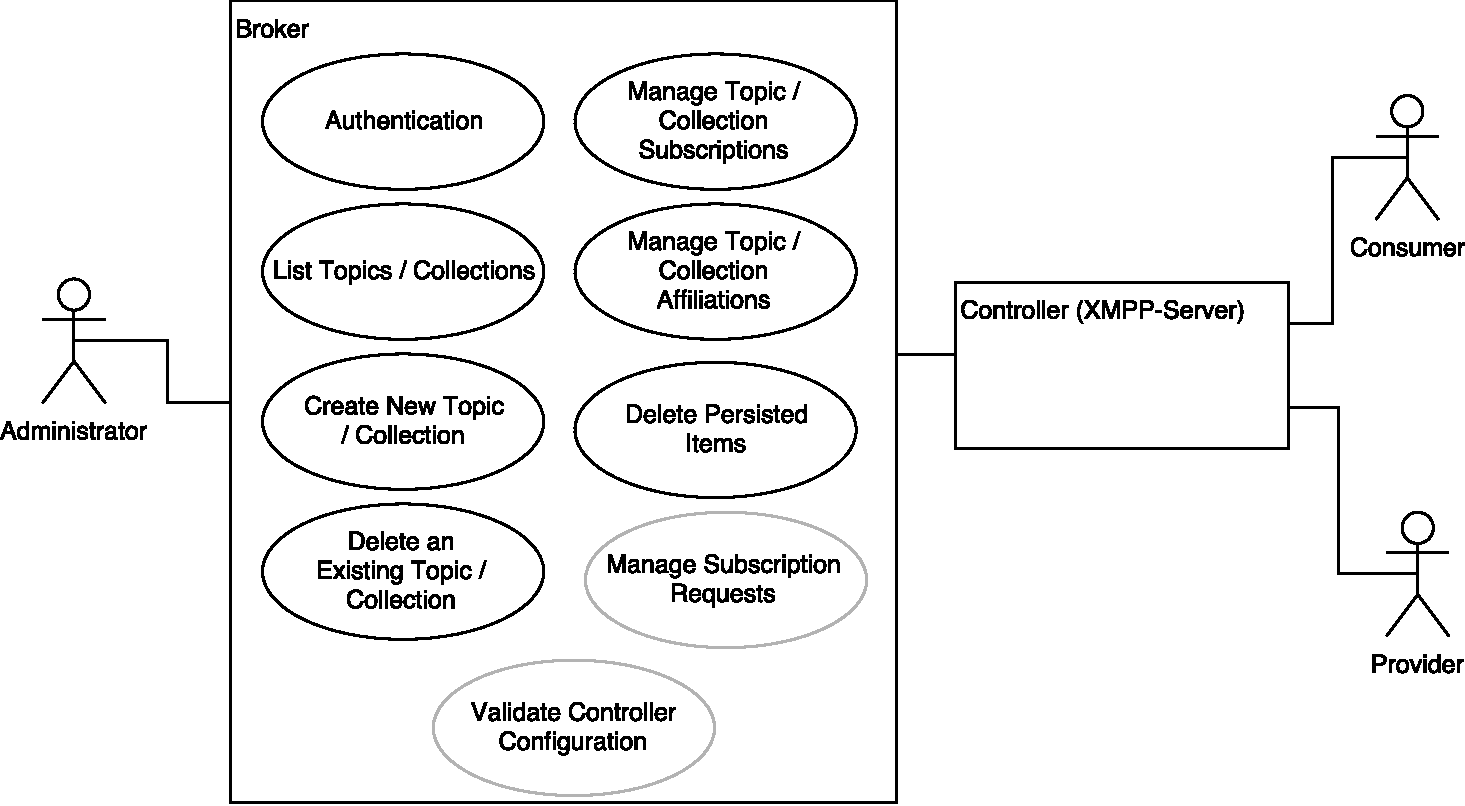
\includegraphics[width=1\linewidth]{resources/requirements_overview}
    \caption[Use case diagram]{UML use case diagram presenting an overview of the primary user stories.}
    \label{fig:requirements-overview}
\end{figure}

\subsection{Authentication}\label{sec:authentication}
\subsubsection{Login}

As an Administrator,\\
I want to log in\\
- preferably using an existing client \gls{tls} certificate - \\
so that only I can inspect and manage topics.\\

\subsubsection{Secure \gls{xmpp} Authentication}

As an Administrator concerned with security requirements,\\
I want to use either \gls{sasl-external} or \gls{sasl-scram} mechanism for authentication -

\begin{itemize}
    \item preferably the SCRAM-SHA-256-PLUS variant and
    \item preferably using mutual certificate-based authentication including revocation status checking
\end{itemize}

\noindent - so that the controller is fully compatible with the \gls{xmpp-grid-standard}~\cite{ietf-mile-xmpp-grid-05}.

\noindent To achieve this goal, I am willing to accept:
\begin{itemize}
    \item More costly and less user friendly authentication
    \item limited compatibility of supported \gls{xmpp} servers
\end{itemize}

\subsubsection{Secure \gls{xmpp} Connection}

As an Administrator concerned with security requirements,\\
I want to use minimally \gls{tls} 1.2 [RFC5246] to communicate with the \gls{xmpp} server at all times\\
to achieve maximal security and compatibility with the \gls{xmpp-grid-standard}~\cite{ietf-mile-xmpp-grid-05}.

\subsubsection{Secure Connection}

As an Administrator concerned with security requirements,\\
I want to use minimally \gls{tls} 1.2 [RFC5246] to communicate with the \gls{broker}\\
to achieve maximal security.

\subsubsection{Multiple Administrators}\label{sec:requirement-multiple-administrators}

As an Administrator,\\
I want to grant access to administrators \\
so that they can also manage the application.

\subsubsection{Audit Trail}\label{sec:requirement-audit-trail}

As an Administrator concerned with security requirements,\\
I want to be able to access an audit log\\
- preferably using existing \gls{xmpp} mechanisms - \\
so that I can reconstruct what other Administrations did on the controller.

\subsubsection{Logout}\label{sec:requirement-logout}

As an Administrator,\\
I want to log out\\
so that I can terminate a session.

\subsection{List Topics and Collections}\label{sec:list-topics}

\subsubsection{List All Topics}\label{sec:requirement-list-all-topics}
As an Administrator,\\
I want to see a list of all topics of the associated controller\\
so that I can quickly assimilate which topics exist.

\subsubsection{List All Top-Level-Collections}
As an Administrator,\\
I want to see a list of all top-level-collections of the associated controller\\
so that I can quickly assimilate which collections exist.

\subsubsection{List All Parent-Collections of a Topic}
As an Administrator,\\
I want to see a list of all transitive parent collections that contain a given topic\\
so that I can quickly assimilate in which collections items are published.

\subsubsection{List All Subtopics and Subcollection of a Collection}
As an Administrator,\\
I want to see a list of all collections and topics that a given collection contains\\
so that I can quickly assimilate the collection hierarchy.

\subsubsection{List Available topics With Limited Access (optional)}

As an Administrator,\\
I want to see a list of all topics of the associated controller to which I have limited access to,\\
to simplify troubleshooting and locate errors.

\subsubsection{List Available collections With Limited Access (optional)}

As an Administrator,\\
I want to see a list of all collections of the associated controller to which I have limited access to,\\
to simplify troubleshooting and locate errors.

\subsubsection{Topic and Collection Paging}
As an Administrator,\\
I want to be able to page through any set of collection/topic with more than 10 Items \\
so that I can work with more than 1000 collections and topics more effectively.

\subsubsection{Topic and Collection Name Filter}\label{sec:requirement-topic-filter}
As an Administrator,\\
I want to be able to quickly filter any set of collections/topics with more than 10 Items \\
so that I can work with more than 1000 collections and topics more effectively.

\subsection{Create a New Topic}\label{sec:create-topic}

As an Administrator,\\
I want to create a new topic on the associated controller\\
so that I am not tied to a fixed set of topics.

\subsection{Create a New Collection}\label{sec:create-collection}

As an Administrator,\\
I want to create a new collection on the associated controller\\
so that I can flexibly patch topics together.

\subsubsection{Override Default Topic Configuration}\label{sec:requirement-topic-default-configuration}

As an Administrator in the process of creating a new topic,\\
I want to override the default configuration (e.g. the affiliations) \\
so that I can restrict access and provide reasonable defaults.

\subsubsection{Override Default Collection Configuration}\label{sec:requirement-collection-default-configuration}

As an Administrator in the process of creating a new collection,\\
I want to override the default configuration (e.g. the affiliations) \\
so that I can restrict access and provide reasonable defaults.

\subsubsection{Initial topic Consumers and Providers}\label{sec:requirement-initial-topic-consumer-provider}

As an Administrator in the process of creating a new topic,\\
I want to specify an initial set of consumers and providers \\
so that I can restrict access to that topic and provide reasonable defaults.

\subsubsection{Initial Collection Consumers}\label{sec:requirement-initial-collection-consumer}

As an Administrator in the process of creating a new collection,\\
I want to specify an initial set of consumers \\
so that I can restrict access to that collection and provide reasonable defaults.

\subsection{Delete an Existing Topic}\label{sec:delete-topic}

As an Administrator,\\
I want to delete an existing topic on the associated controller\\
so that I can get rid of obsolete topics.

\subsection{Delete an Existing Collection}\label{sec:delete-collection}

As an Administrator,\\
I want to delete an existing collection on the associated controller\\
so that I can get rid of obsolete collections.


\subsubsection{Fault Prevention On Topic-Delete}

As an Administrator in the process of deleting a topic, \\
I want a mechanism to prevent me from deleting the wrong topic on the associated controller\\
(e.g. require me to enter the name of the topic manually).

\subsubsection{Fault Prevention On Collection-Delete}

As an Administrator in the process of deleting a collection, \\
I want a mechanism to prevent me from deleting the wrong collection on the associated controller\\
(e.g. require me to enter the name of the collection manually).


\subsection{Manage Topic/Collection Subscriptions}\label{sec:manage-subscriptions}

\subsubsection{List Consumers}

As an Administrator, \\
I want to list all consumers (including their JIDs) of a given topic/collection on the associated controller, \\
so that I can verify that specific consumers are subscribed, and others are not.


\subsubsection{Inspect Detailed Subscription Configuration}

As an Administrator, \\
I want to inspect the detailed topic/collection subscription configuration of a given consumer, \\
so that I can reproduce and reason about the receipt of data on that consumer
and find potential misconfiguration.

\subsubsection{Partially Modify Subscription Configuration}

As an Administrator, \\
I want to modify parts of the topic/collection subscription configuration of a given consumer, \\
so that I can fix misconfiguration.

\subsubsection{Unsubscribe Consumer}

As an Administrator, \\
I want to manually unsubscribe a specific consumer from a particular topic/collection on the associated controller, \\
so that I can remove obsolete or undesired subscriptions.

\subsubsection{Subscribe Consumer}

As an Administrator, \\
I want to manually subscribe a specific consumer on a particular topic/collection on the associated controller, \\
so that I can faster setup and manage consumers.

\subsection{Manage Topic Affiliations}\label{sec:manage-affiliations}
\subsubsection{Inspect Affiliations}

As an Administrator,\\
I want to list all Affiliations (JID and "Role") for a particular topic/collection on the associated controller \\
so that I can find potential misconfiguration.

\subsubsection{Modify Affiliations}

As an Administrator,\\
I want to modify the Affiliation ("Role") of a given JID for a particular topic/collection on the associated controller \\
so that I can fix potential misconfiguration.

\subsubsection{Fault Prevention When Modifying My Affiliation}

As an Administrator in the process of modifying my Affiliation for a particular topic/collection on the associated controller,\\
I want a mechanism to prevent me from accidentally downgrading my rights.

\subsubsection{Meaningful Error For Topics/Collection With Limited Access}

As an Administrator,\\
I want to receive a meaningful error message when inspecting a topic/collection to which I have limited access \\
so that I can quickly comprehend why the configuration options are limited.

\subsection{Manage Persisted Items of a Topic}\label{sec:manage-persisted-items}
\subsubsection{Inspect Persisted Items}

As an Administrator,\\
I want to list all persisted items for a particular topic on the associated controller \\
so that I can get an overview and check for misconfiguration.

\subsubsection{Filter Persisted Items}\label{sec:requirement-filter-persisted-items}

As an Administrator,\\
I want to be able to filter all persisted items of a specific topic by \\
\begin{itemize}
    \item the timestamp of its publication
    \item the publishers JID
\end{itemize}
so that I can work with more than 10000 persisted items more effectively.

\subsubsection{Paged Persisted Items}\label{sec:paged-persisted-items}
As an Administrator working with filtered persisted items,\\
I want to be able to page through the resulting items\\
- given that this feature is supported by the associated controller -\\
so that I can work with more than 10000 persisted items more effectively.

\subsubsection{Delete a Persisted Items From a Topic}

As an Administrator,\\
I want to delete a particular persisted item from a specific topic\\
- given that this feature is supported by the associated controller -\\
so that I can clean up test items and remove obsolete or corrupted items.

\subsubsection{Purge All Persisted Items From a Topic}

As an Administrator,\\
I want to purge persisted items from a specific topic\\
- given that this feature is supported by the associated controller -\\
so that I can clean up test items and remove obsolete or corrupted items.

\subsubsection{Delete Set of Persisted Items From a Topic (optional)}

As an Administrator,\\
I want to delete a set of persisted item that match a given criteria from a specific topic\\
- given that this feature is supported by the associated controller -\\
so that I can clean up test items and remove obsolete or corrupted items.

\subsection{Manage Subscription Requests (optional)}\label{sec:subscription-requests}

\subsubsection{List Subscription Request}
As an Administrator,\\
I want to list pending subscription requests for a given topic\\
- given that this feature is supported by the associated controller -\\
so that I can quickly assimilate pending requests.

\subsubsection{Accept Subscription Request}

As an Administrator,\\
I want to accept a pending subscription request for a given topic\\
- given that this feature is supported by the associated controller -\\
to enable more dynamic access models than just maintaining a black- or whitelist.

\subsubsection{Reject Subscription Request}

As an Administrator,\\
I want to reject a pending subscription request for a given topic\\
- given that this feature is supported by the associated controller -\\
so that I can deny user access in accordance with the \gls{xmpp} standards.

\subsection{Validate Controller Configuration (optional)}\label{sec:validate-controller-config}

\subsubsection{Validate Supported XEPs Configurations}
As an Administrator,\\
I want to validate that a minimum set of XEPs are supported by the associated controller\\
so that I can quickly identify incompatibilities.

\subsubsection{Validate Optional XEP Implementations}
As an Administrator,\\
I want to validate that the required features that are marked as optional or recommended in the XEPs are implemented by the associated controller\\
so that I can quickly identify incompatibilities.


% !TeX spellcheck = en_GB

\section{Wireframes}\label{sec:wireframes}

\begin{figure}[h]
    \centering
    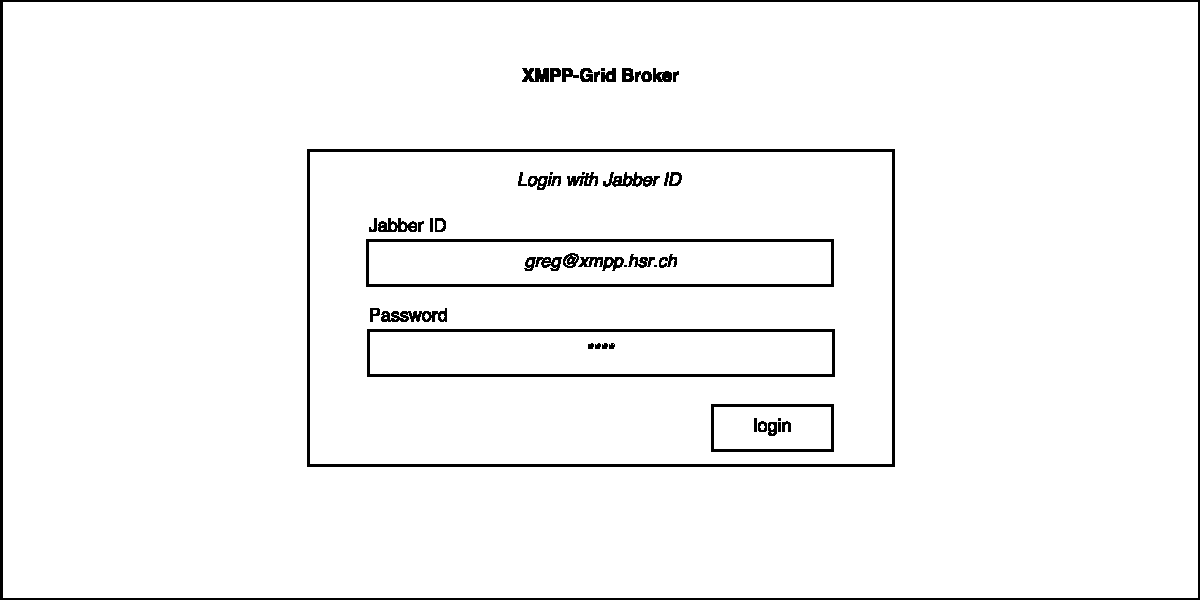
\includegraphics[width=1\linewidth]{resources/wireframe_1}
    \caption{Login-screen wireframe}
\end{figure}

\begin{figure}[h]
    \centering
    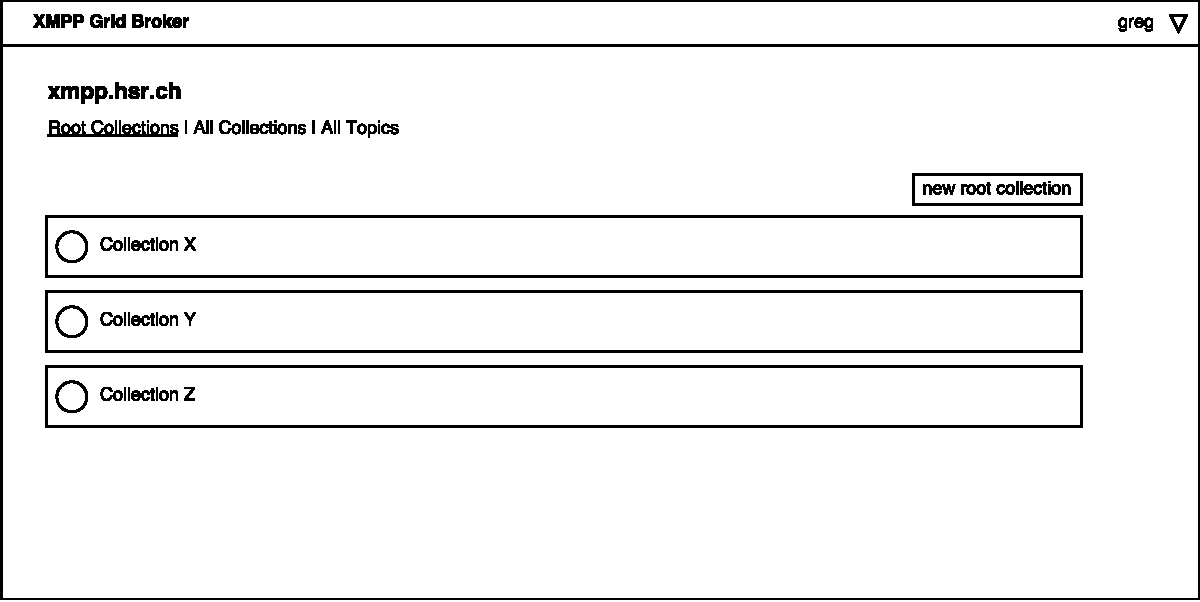
\includegraphics[width=1\linewidth]{resources/wireframe_2}
    \caption{Controller overview wireframe}
\end{figure}

\begin{figure}[h]
    \centering
    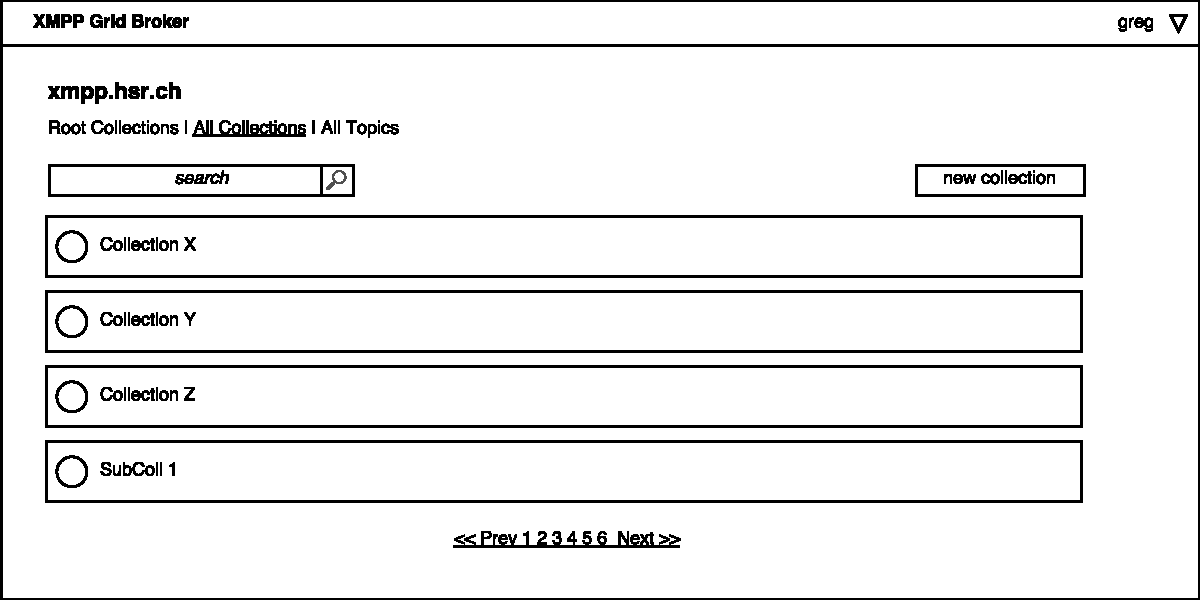
\includegraphics[width=1\linewidth]{resources/wireframe_3}
    \caption{All collections wireframe}
\end{figure}

\begin{figure}[h]
    \centering
    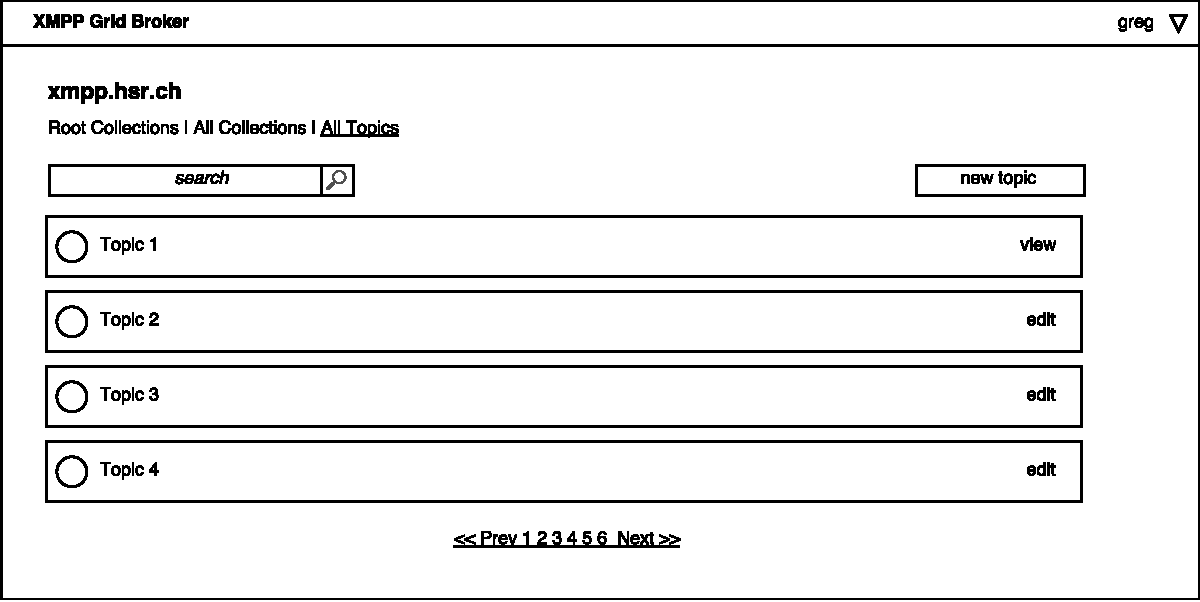
\includegraphics[width=1\linewidth]{resources/wireframe_4}
    \caption{All topics wireframe}
\end{figure}

\begin{figure}[h]
    \centering
    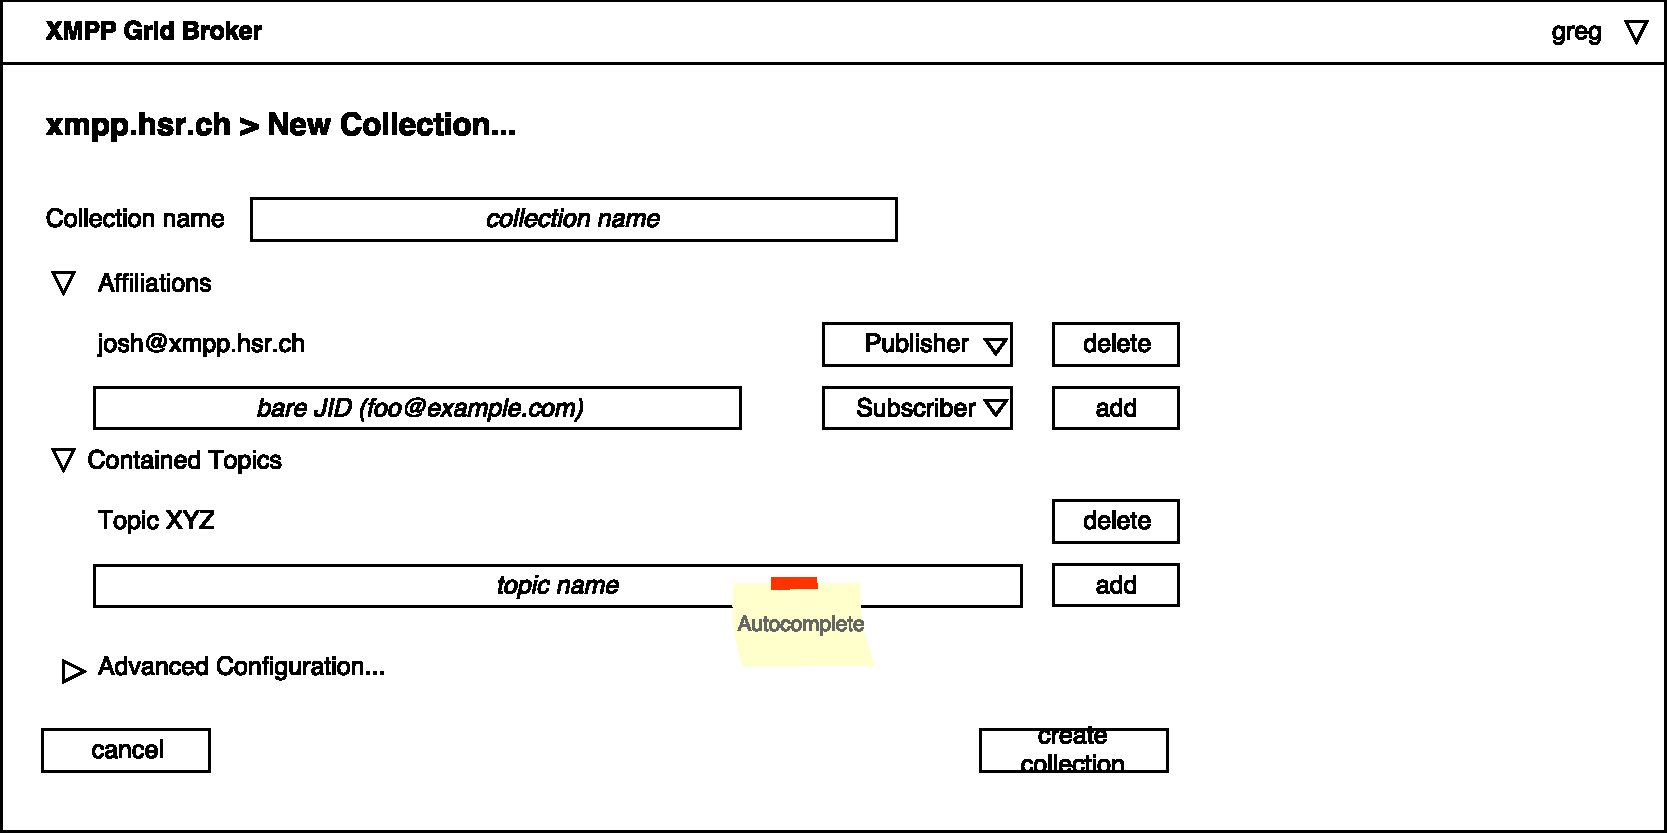
\includegraphics[width=1\linewidth]{resources/wireframe_5}
    \caption{New collection wireframe}
\end{figure}

\begin{figure}[h]
    \centering
    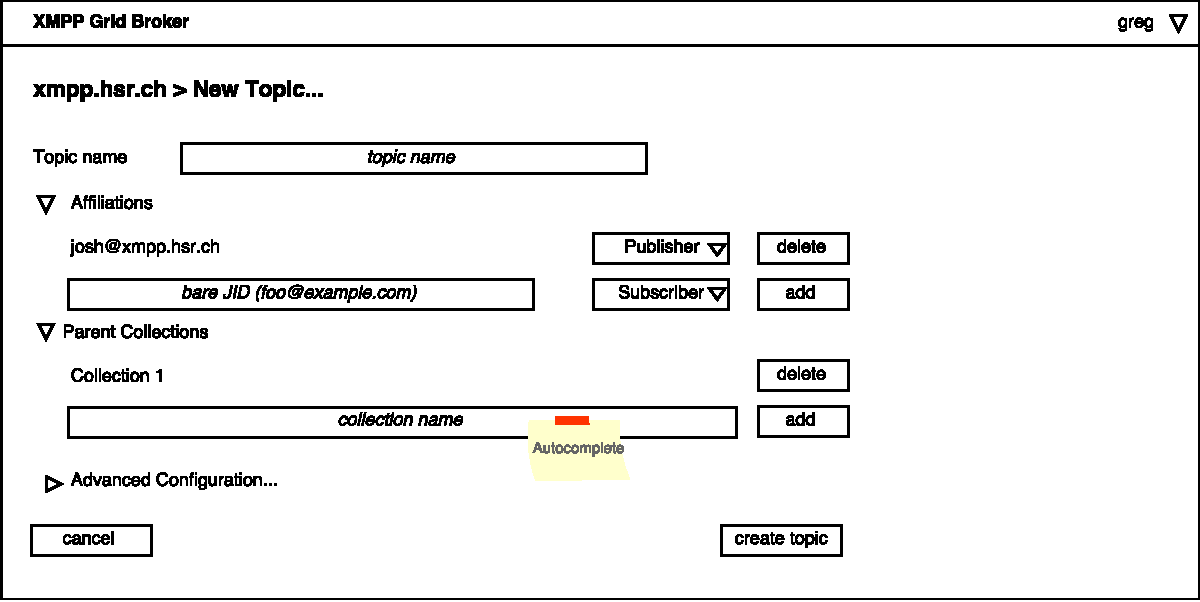
\includegraphics[width=1\linewidth]{resources/wireframe_6}
    \caption{New topic wireframe}
\end{figure}

\begin{figure}[h]
    \centering
    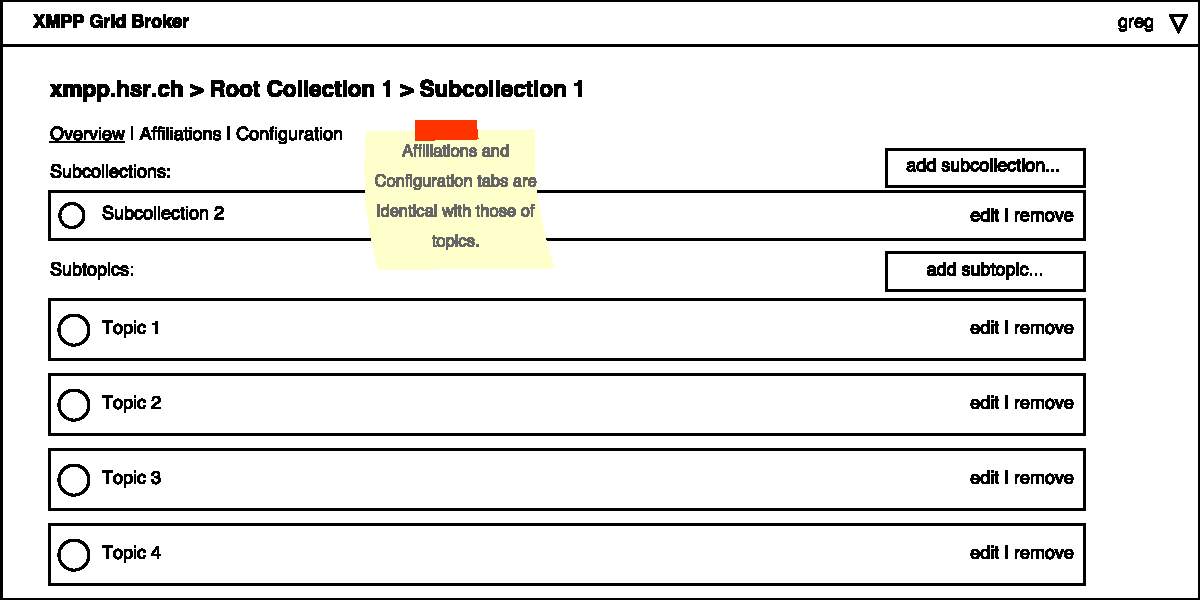
\includegraphics[width=1\linewidth]{resources/wireframe_7}
    \caption{Collection overview wireframe}
\end{figure}

\begin{figure}[h]
    \centering
    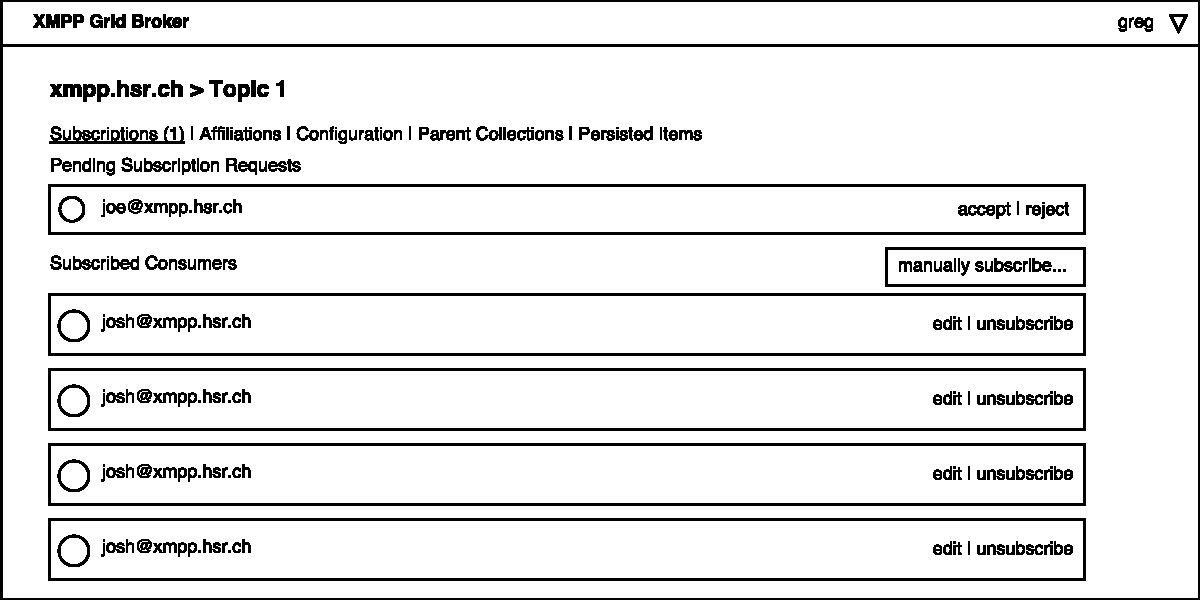
\includegraphics[width=1\linewidth]{resources/wireframe_8}
    \caption{Topic overview wireframe}
\end{figure}

\begin{figure}[h]
    \centering
    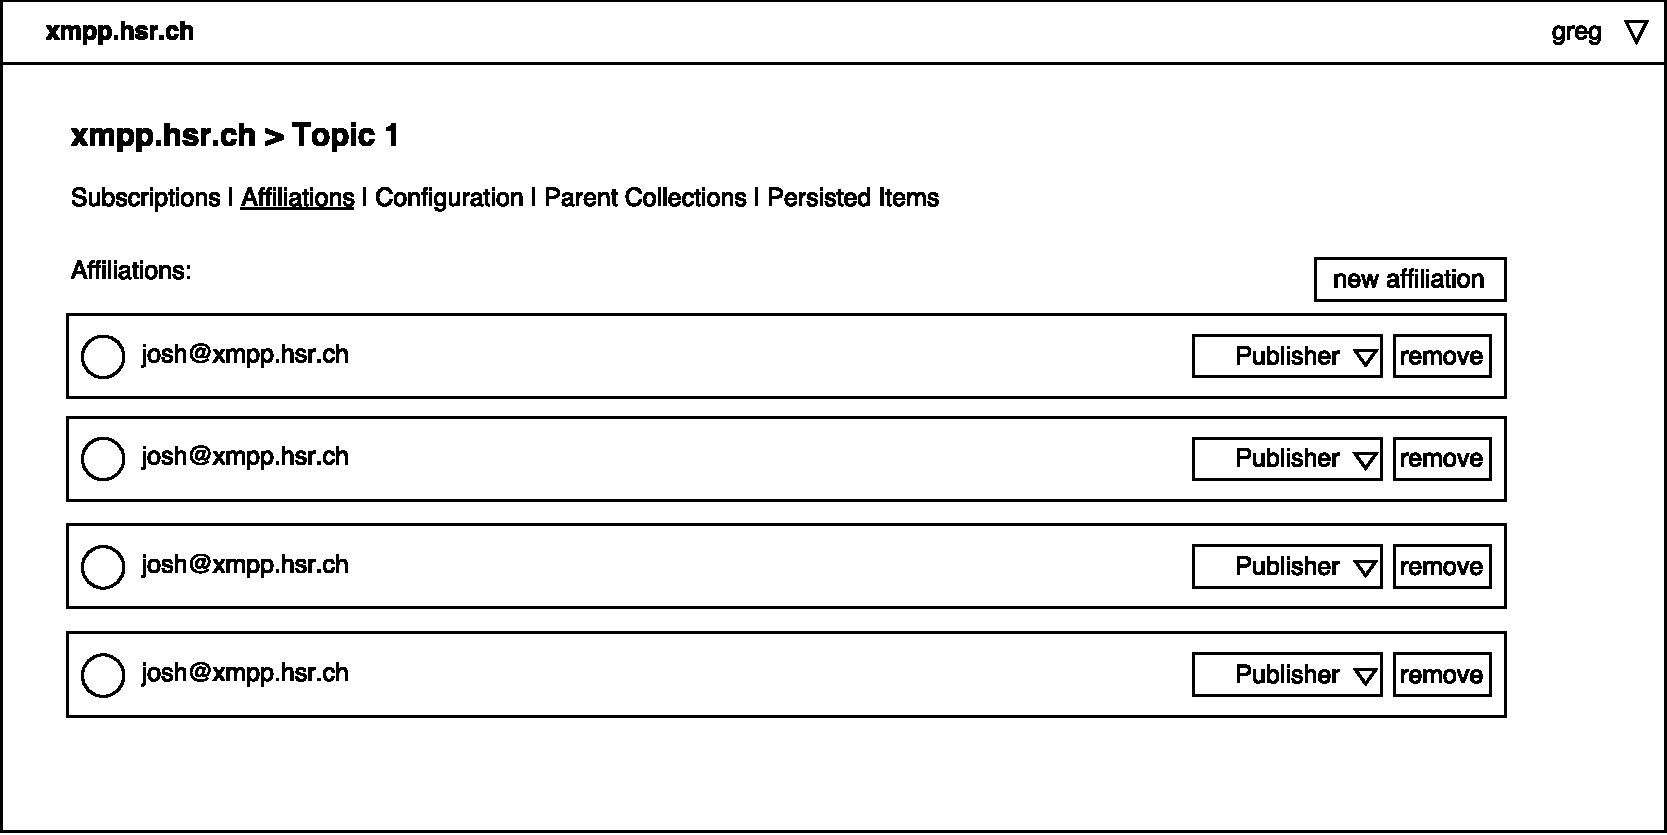
\includegraphics[width=1\linewidth]{resources/wireframe_9}
    \caption{Topic/Collection affiliations wireframe}
\end{figure}

\begin{figure}[h]
    \centering
    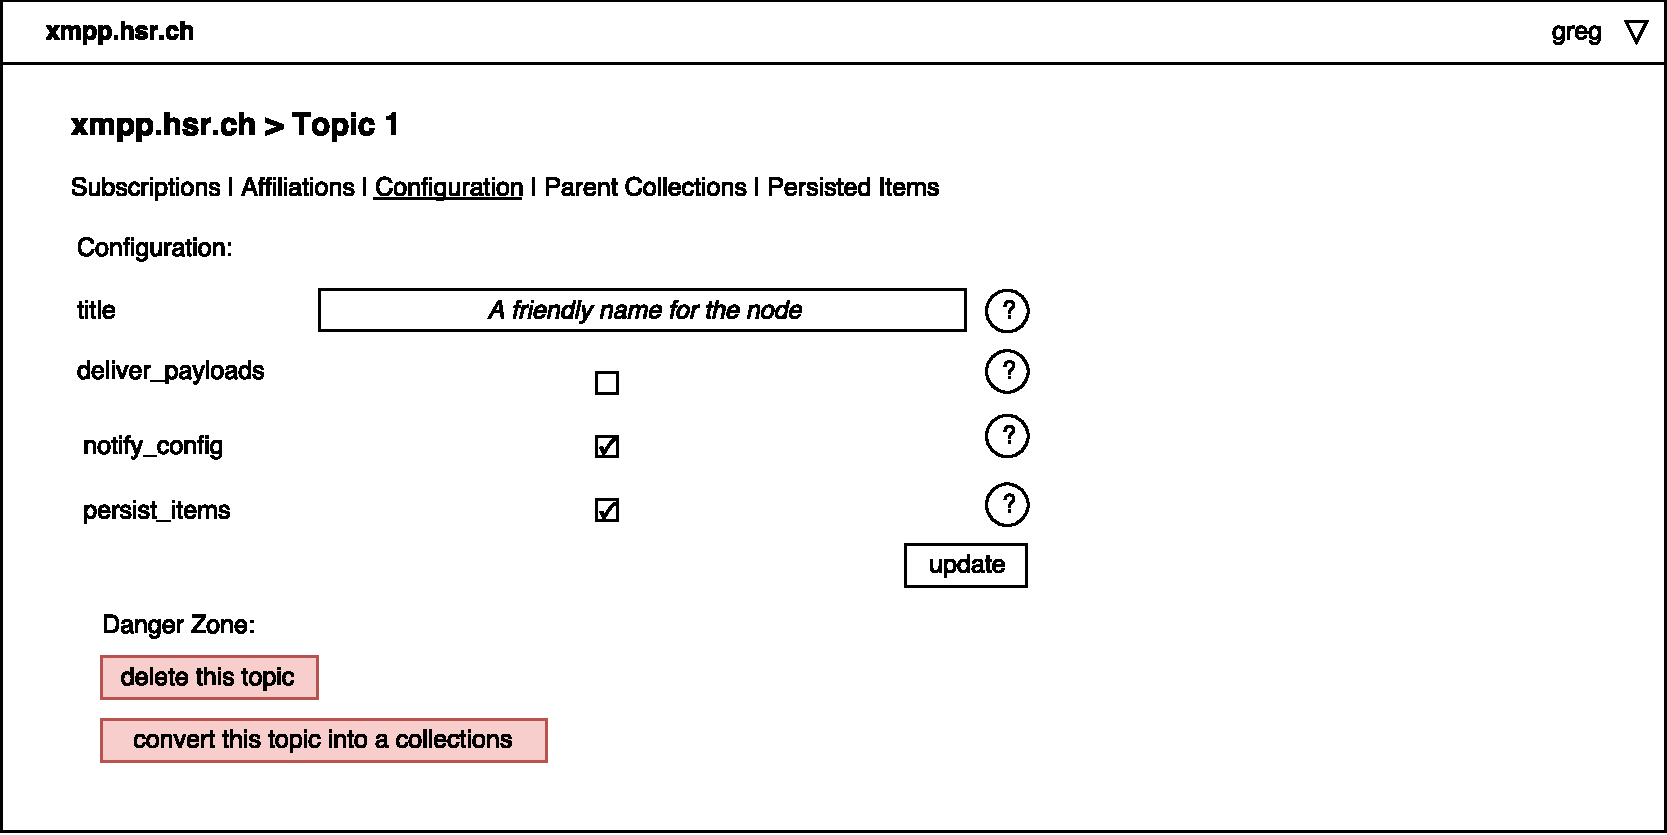
\includegraphics[width=1\linewidth]{resources/wireframe_10}
    \caption{Topic/Collection configuration wireframe}
\end{figure}

\begin{figure}[h]
    \centering
    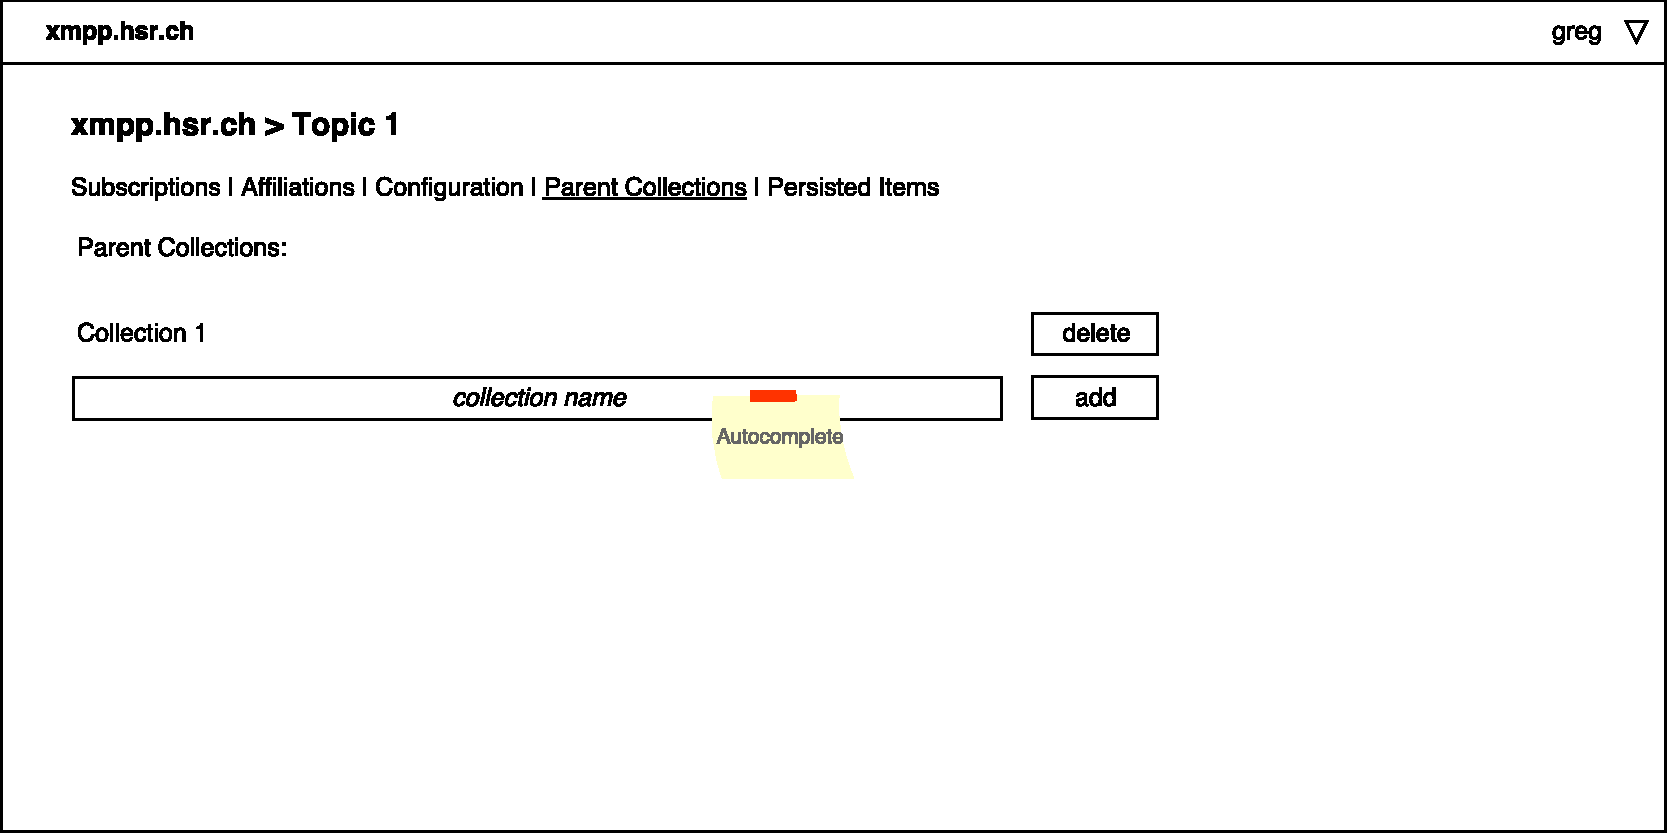
\includegraphics[width=1\linewidth]{resources/wireframe_11}
    \caption{Topic parent collections items wireframe}
\end{figure}

\begin{figure}[h]
    \centering
    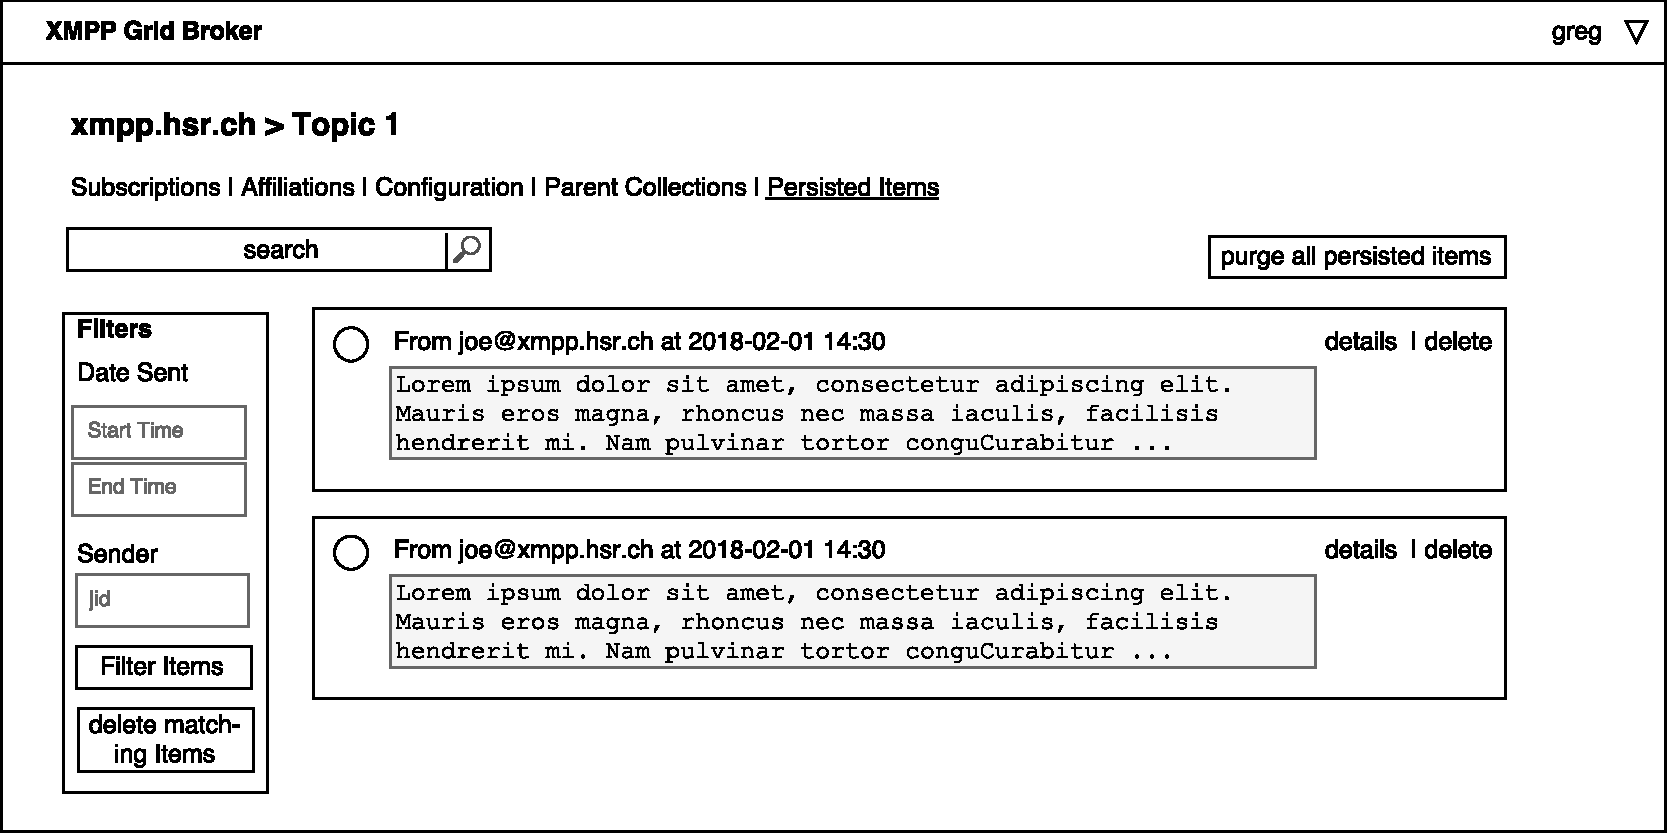
\includegraphics[width=1\linewidth]{resources/wireframe_12}
    \caption{Persisted items wireframe}
\end{figure}
% !TeX spellcheck = en_GB
\section{Comparison of XMPP Server and Libraries}\label{sec:comparison-of-xmpp-server-and-libraries}


\subsection{Server}

To find a suited server to develop, test and document our application with, we considered the three major open source \gls{xmpp} servers, which are still under active maintenance and provide extensive documentation on their XEP-implementations.

For our implementation, we might require the following XEPs respectively RFCs. Any deviations are noted under ``XEP/RFC Support''.

\begin{description}
    \item[XEP-0004] Data Forms
    \item[XEP-0030] Service Discovery
    \item[XEP-0059] Result Set Management
    \item[XEP-0060] Publish-Subscribe
    \item[XEP-0114] Jabber Component Protocol
    \item[XEP-0133] Service Administration
    \item[XEP-0178] Best Practices for Use of SASL EXTERNAL with Certificates
    \item[XEP-0206] XMPP Over BOSH
    \item[XEP-0248] PubSub Collection Nodes
    \item[RFC-7395] An XMPP Subprotocol for WebSocket
\end{description}

\subsubsection{Openfire}
\begin{tabu}{l X}
    Programming Language
    & Java \\

    Plugin Architecture
    & Java JAR\footnote{\url{http://download.igniterealtime.org/openfire/docs/latest/documentation/plugin-dev-guide.html}} \\

    XEP/RFC Support
    & \begin{tabu}{@{}l X}
    XEP-0133 & Partial, also not explicitly supported\footnote{\url{https://issues.igniterealtime.org/browse/OF-284}}\\
    XEP-0178 & Partial, also not explicitly supported\footnote{\url{https://github.com/Connectify/Openfire/blob/master/src/java/org/jivesoftware/openfire/net/SASLAuthentication.java} and \hfill\\ \url{https://issues.igniterealtime.org/browse/OF-1191}}\\
    XEP-0248 & Partial, as part of outdated XEP-0060\footnote{\url{https://igniterealtime.jiveon.com/thread/38929}} \\
    \end{tabu}
    All other required XEPs are supported\footnote{\url{http://download.igniterealtime.org/openfire/docs/latest/documentation/protocol-support.html}}\\

\end{tabu}

\subsubsection{Prosody}
\begin{tabu}{l X}
    Programming Language
    & Lua \\

    Plugin Architecture
    & Luascript\footnote{\url{https://prosody.im/doc/developers/modules}} \\

    XEP/RFC Support
    & \begin{tabu}{@{}l X}
    XEP-0059 & Not supported\\
    XEP-0178 & Not supported\\
    XEP-0248 & Not supported\\
    \end{tabu}
    All other required XEPs are supported\footnote{\url{https://prosody.im/doc/modules} and  \url{https://prosody.im/doc/xeplist}}\\
\end{tabu}

\subsubsection{Ejabberd}
\begin{tabu}{l X}
    Programming Language
    & Erlang \\

    Plugin Architecture
    & Erlang/Elixir\footnote{\url{https://docs.ejabberd.im/developer/extending-ejabberd/modules/}} \\

    XEP/RFC Support
    & \begin{tabu}{@{}l X}
    XEP-0178 & Partial, commercially only\footnote{Server to server only in community edition}\\
    RFC-7395 & Partial, not explicitly supported\footnote{\url{https://docs.ejabberd.im/xmpp}}\\
    \end{tabu}
    All other required XEPs are supported\footnote{\url{http://www.ejabberd.im/protocols}} \\
\end{tabu}

\subsection{Libraries}

To find a suited library to implement our application with, we considered various open source \gls{xmpp} libraries, which are still under active maintenance and provide extensive documentation on their XEP-implementations. We also limited the programming languages to Python, Java and JavaScript as discussed in the project meeting of 2018-03-05 (see~\fullref{sec:meeting-minutes}).

For our implementation, we might require the following XEPs. Any deviations are noted under ``Limitations''.

\begin{description}
    \item[XEP-0004] Data Forms
    \item[XEP-0030] Service Discovery
    \item[XEP-0059] Result Set Management
    \item[XEP-0060] Publish-Subscribe
    \item[XEP-0114] Jabber Component Protocol
    \item[XEP-0133] Service Administration
    \item[XEP-0178] Best Practices for Use of \gls{sasl-external} with Certificates
    \item[XEP-0206] \gls{xmpp} Over \gls{bosh}
    \item[XEP-0248] PubSub Collection Nodes
    \item[RFC-7395] An \gls{xmpp} Subprotocol for WebSocket (mentioned only if differs from XEP-0206 implementation status)
\end{description}

\begin{tabu}{l|l l X}
    \hline
    Name
    & Language
    & Plugins
    & Limitations
    \\ \hline

    SleekXMPP\footnote{\url{http://sleekxmpp.com/xeps.html}}
    & Python 2
    & Yes\footnote{\url{http://sleekxmpp.com/create_plugin.html}}
    & \textbf{Not Supported:} XEP-114, XEP-133, XEP-248, XEP-0206\newline
    \textbf{Partial:} XEP-0060\footnote{Client-side only}
    \\

    SliXMPP\footnote{\url{https://github.com/poezio/slixmpp/blob/master/docs/xeps.rst}}
    & Python 3
    & Yes\footnote{\url{https://github.com/poezio/slixmpp/blob/master/docs/create_plugin.rst}}
    & \textbf{Not Supported:} XEP-114, XEP-133, XEP-248, XEP-0206\newline
    \textbf{Partial:} XEP-0060\footnote{Client-side only}
    \\

    aioxmpp\footnote{\url{https://docs.zombofant.net/aioxmpp/devel/\#from-xmpp-extension-proposals-xeps}}
    & Python 3.4
    & Yes\footnote{\url{https://docs.zombofant.net/aioxmpp/devel/api/public/index.html\#apis-mainly-relevant-for-extension-developers}}
    & \textbf{Not Supported:} XEP-0114, XEP-0133, XEP-0178, XEP-248, XEP-0206
    \\

    Smack\footnote{\url{https://download.igniterealtime.org/smack/docs/latest/documentation/extensions/index.html}}
    & Java
    & Yes\footnote{\url{https://github.com/igniterealtime/Smack/tree/master/documentation}}
    & \textbf{Not Supported:} XEP-0114, XEP-0206
    \\

    Babbler\footnote{\url{https://sco0ter.bitbucket.io/babbler/xeps.html}}
    & Java
    & Yes\footnote{\url{https://sco0ter.bitbucket.io/babbler/customextensions.html}}
    & \textbf{Not Supported:} XEP-0133, XEP-0248
    \\

    XMPP-FTW\footnote{\url{http://docs.xmpp-ftw.org/manual/}}
    & JS(Browser)
    & Yes\footnote{\url{http://docs.xmpp-ftw.org/}}
    & \textbf{Not Supported:}\newline XEP-0114, XEP-0133, XEP-0248\newline
    \textbf{Unclear:} XEP-0206, XEP-0178\newline
    \textbf{Note:} Requires Server Abstraction
    \\

    Stanza.io\footnote{\url{https://github.com/legastero/stanza.io/blob/master/docs/Supported_XEPs.md}}
    & JS(Browser)
    & Yes\footnote{\url{https://github.com/legastero/stanza.io/blob/master/docs/Create_Plugin.md}}
    & \textbf{Not Supported:}\newline XEP-0114, XEP-0133, XEP-0248\newline
    \textbf{Partial:} XEP-0178\footnote{Not explicitly supported}
    \\

    strophe.js\footnote{\url{https://github.com/strophe/strophejs-plugins}}
    & JS(Browser)
    & Yes\footnote{\url{https://github.com/strophe/strophejs-plugins}}
    & \textbf{Not Supported:}\newline XEP-0114, XEP-0133, XEP-0248\newline
    \textbf{Partial:} XEP-0178\footnote{Not explicitly supported}
\end{tabu}

% !TeX spellcheck = en_GB
\section{Personal Reports}\label{sec:personal-reports}

\subsection{Raphael Zimmermann}

This project was an exciting journey for me because I wasn't familiar with the subject matter and the XMPP protocol at all.

I was surprised that many of the XEPs we used were still in a draft state even though they were around for over ten years and implemented in most servers.
It was even more surprising to me that these XEPs were modified significantly, contradicting my wishful thinking to rely on the specification entirely.
I also learned, that having too many optional features in a standard makes working with it tedious, especially if this functionality seems pivotal.

Because I had no prior experience with Angular, it took much work to understand all relevant underlying concepts.
In hindsight, I must admit that I underestimated the complexity and familiarisation period.
As a result, I was shifting my focus unintentionally from other practices that I usually focus on, such as clean layering.
Nonetheless, I am glad to get familiar with Angular and I mostly enjoyed working with it.

Fabian and I are a well-practised team and as in our study project, working together was a pleasure.

\subsection{Fabian Hauser}

\beautyquote{The important thing is not to stop questioning.}{Albert Einstein}
%
I find this quote very fitting for our thesis - not only was it our task to decide on options,
but also keep questioning them to find the best possible solution.

We used architectural design decisions to find and question possible solutions.
This technique supported our problem solving process greatly in my opinion.
The most surprising turn resulting from an architectural decision during the project was our decision to write a client only application,
which I wouldn't have expected from the task description.

During the project, I often had the feeling that we didn't advance as fast as I had hoped for.
I think the main reason for this feeling is the time it took to get familiar with the complex XMPP standards.

Working together with Raphael was a very pleasant experience.
Although we often worked remote from home, we had great discussions and conversations.
Nevertheless, I think that it was helpful that we took the time to meet at least one time a week, which improved our communication and team spirit.

%----------------------------------------------------------------------------------------
%	DECLARATION PAGE
%----------------------------------------------------------------------------------------

\begin{declaration}
\addchaptertocentry{\authorshipname} % Add the declaration to the table of contents
\noindent We, \authorname, declare that this thesis and the work presented in it are our own, original work.  All the sources we consulted and cited are clearly attributed. We have acknowledged all main sources of help. \\

\noindent Fabian Hauser\\[2em]
\rule[0.5em]{25em}{0.5pt}\\ % This prints a line for the signature
\noindent Raphael Zimmermann\\[2em]
\rule[0.5em]{25em}{0.5pt}\\ % This prints a line for the signature 
\noindent Rapperswil, \today
\end{declaration}

\cleardoublepage


%----------------------------------------------------------------------------------------

\end{document}  
